\chapter{Initial Value Problems}

\section{The explicit midpoint rule}

Let \(f: \R\times \R^n \rightarrow \R^n\) be a smooth mapping and consider the initial value problem 
\begin{equation}\label{ivp}
y'(t) = f(t, y(t)), \quad y(a) = y_a, \quad t\in [a,b].
\end{equation}
The explicit midpoint methods is a method for computing an approximation to the solution of (\ref{ivp}), and it goes as follows: Let \(n\geq 1\) be an integer and \(h\coloneqq (b-a)/2n\). We then define recursively
\[
\xi_h(a) \coloneqq y_a, \quad \xi_h(a+h) \coloneqq \xi_h(a) + hf(a, \xi_h(a))
\]
and
\[
\xi_h(a + (i+1)h) \coloneqq \xi_h(a+(i-1)h) + 2hf(a+ih, \xi(a+ih)).
\]
Then \(\xi_h\) is an approximate solution to (\ref{ivp}) defined at \(a, a+h,\ldots ,b\). We are interested in the value \(X_f(h)\coloneqq \xi_h(b)\). It is possible to show that \(X_f(h)\) has an asymptotic expansion in \(h^2\). We have the following implementation in Python of the explicit midpoint rule for computing \(X_f(h)\).

\begin{minted}[tabsize=2, fontsize=\footnotesize]{python}
class ExplicitMidpointRule(Scheme):

	def __init__(self):
		super(ExplicitMidpointRule, self).__init__(2)

	def apply(self, ivp, n):
		h = (ivp.b - ivp.a) / (2 * n)
		y_sl = ivp.y0
		y_l = ivp.y0 + h * ivp.f(ivp.a, ivp.y0)

		for i in range(1, 2 * n):
			tmp = y_l
			y_l = y_sl + 2 * h * ivp.f(ivp.a + i * h, y_l)
			y_sl = tmp

		return y_l
\end{minted}

\section{Numerical experiments}

In this section we are going to extrapolate the explicit midpoint rule and analyze the convergence of the approximations as we extrapolate more often. Consider the initial value problem (\ref{ivp}). Let \(n_1 < n_2 < \cdots\) be some sequence of integers and \(h_i \coloneqq (b-a) / n_i\). Let \(X_{ij}\) the extrapolation table which we get from extrapolating in \(h^2\), using the points \((h_i,X_f(h_i))\). Let \(\varepsilon_i \coloneqq |X_{ii} - y(b)|\) be the absolute error. We are going to do the same convergence and efficency analysis as in the two previous chapters. We will both do the computations using high precision arithmetic with \(500\) correct digits and also in standard double precision.\\

%If \((a_n)\) is the sequence we use then the number of \(f\)-evaluations is %\(N_n = \sum_{k=1}^n 2\cdot a_n\). Thus for the harmonic sequence we have %\(N_n = n(n+1) \approx n^2\) for \(n\) large so if \(\varepsilon_n \sim %A\exp (-cN_n^q)\) then \(\varepsilon_n \sim A\exp(-cn^{2q})\) for large %\(n\). For the Romberg sequence then \(N_n = 2^{n+1} - 1\) so if %\(\varepsilon_n\sim A\exp(-cN_n^q)\) then \(\varepsilon_n \sim %A\exp(-c2^{nq})\) for large \(n\).\\

In those cases where we do not have an analytic solution to the equations, we computed a reference solution up to \(500\) significant digits. We did that by using extrapolation with the harmonic sequence and estimating the error as the difference between successive terms in the sequence of approximations.\\

Now we will consider the results of the experiments.

\subsection{Exponential growth}
First we will consider the following initial value problem:
\begin{equation}\label{42}
y'(x) = y(x),\quad y(0) = 0, \quad x\in [0,1]
\end{equation}
whose solution is the analytic function \(y(x) = e^x\).

\begin{figure}[H]
\centering
\begin{minipage}{0.45\textwidth}
\centering
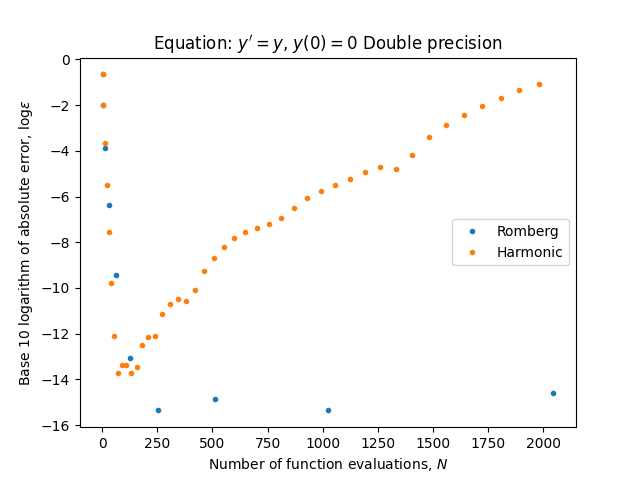
\includegraphics[scale=0.45]{../results/emr_plots/exp_growth.png}
\end{minipage}
\begin{minipage}{0.45\textwidth}
\centering
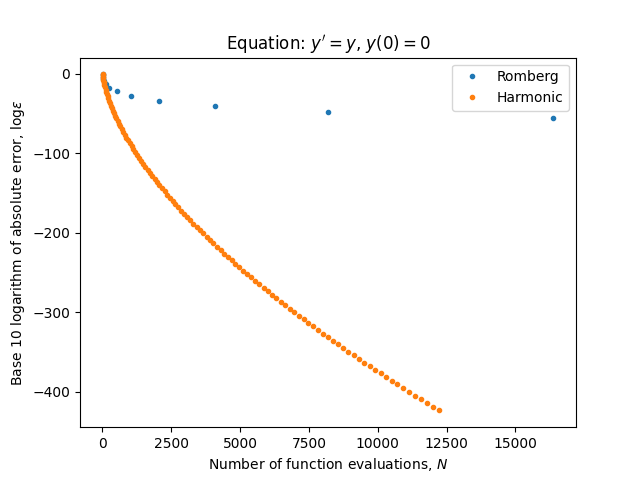
\includegraphics[scale=0.45]{../results/emr_plots/exp_growth_hp.png}
\end{minipage}
\end{figure}

\begin{figure}[H]
\centering
\begin{minipage}{0.45\textwidth}
\centering
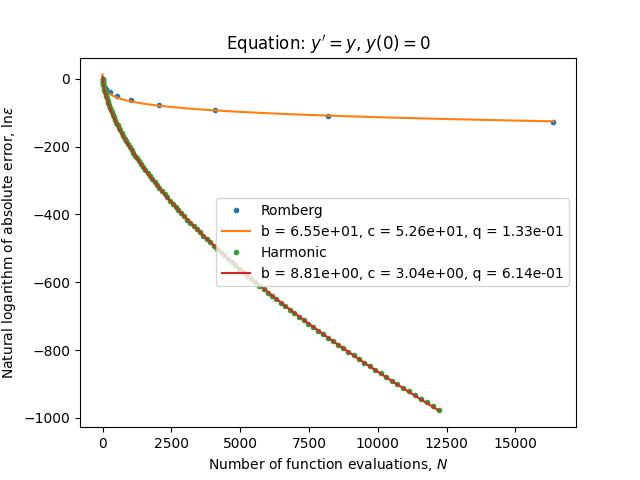
\includegraphics[scale=0.45]{../results/emr_plots/exp_growth_hp_trend.png}
\end{minipage}
\begin{minipage}{0.45\textwidth}
\centering
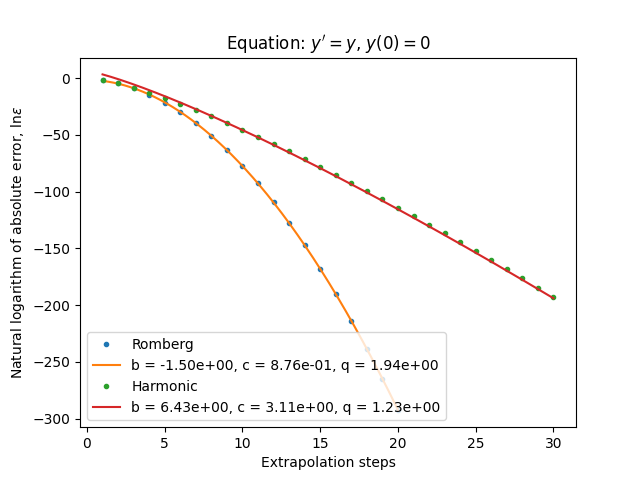
\includegraphics[scale=0.45]{../results/emr_plots/exp_growth_hp_steps.png}
\end{minipage}
\end{figure}

\begin{figure}[H]
\centering
\begin{minipage}{0.45\textwidth}
\centering
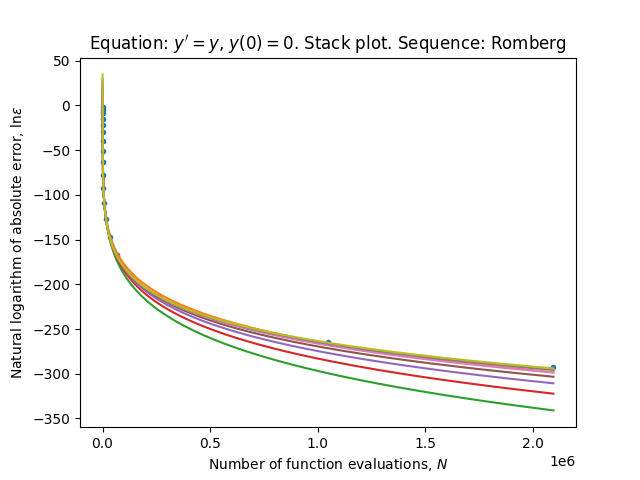
\includegraphics[scale=0.45]{../results/emr_plots/exp_growth_hp_romberg_stack.png}
\end{minipage}
\begin{minipage}{0.45\textwidth}
\centering
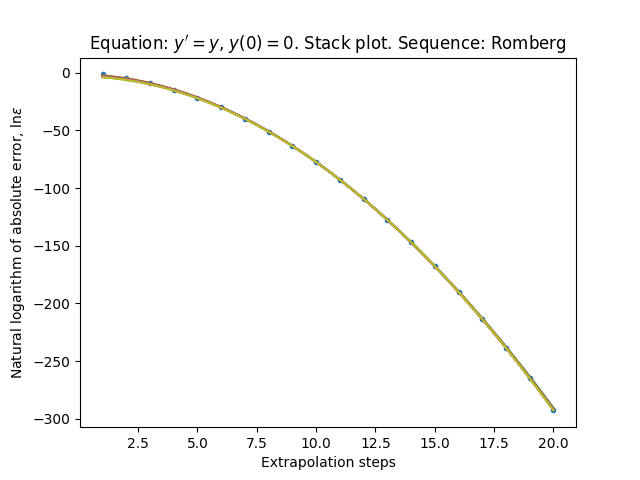
\includegraphics[scale=0.45]{../results/emr_plots/exp_growth_hp_romberg_steps_stack.png}
\end{minipage}
\end{figure}

\begin{figure}[H]
\centering
\begin{minipage}{0.45\textwidth}
\centering
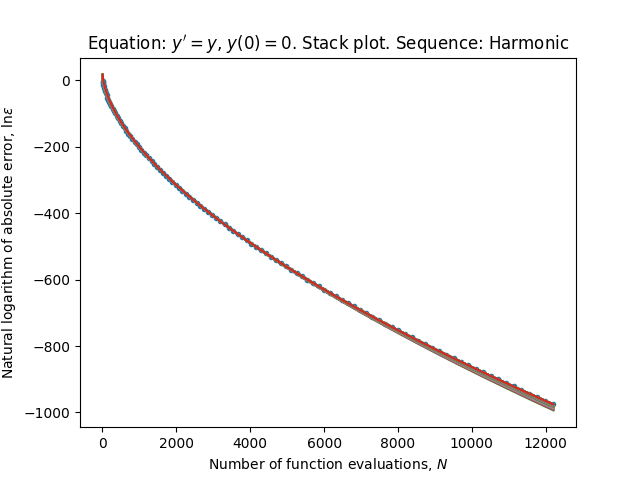
\includegraphics[scale=0.45]{../results/emr_plots/exp_growth_hp_harmonic_stack.png}
\end{minipage}
\begin{minipage}{0.45\textwidth}
\centering
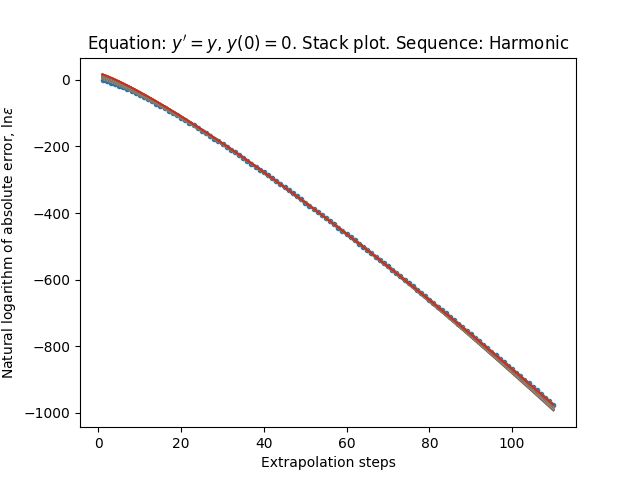
\includegraphics[scale=0.45]{../results/emr_plots/exp_growth_hp_harmonic_steps_stack.png}
\end{minipage}
\end{figure}

\begin{table}[H]
    \centering
    \small
    \begin{tabular}{c|c||c|c|c|c|c|c}
Sequence & Plot & \(A\)-mean & \(A\)-var & \(c\)-mean & \(c\)-var & \(q\)-mean & \(q\)-var\\\hline
\rowcolor{red}
Romberg & lin-ln evals-error & \(6.231\cdot 10^{65}\) & \(6\) & \(71.92\) & \(0.1174\) & \(0.1236\) & \(0.03122\) \\
\rowcolor{yellow}
Harmonic & lin-ln evals-error & \(1.204\cdot 10^9\) & \(6.365\) & \(3.264\) & \(0.005221\) & \(0.6081\) & \(0.0001653\) \\
\rowcolor{green}
Romberg & lin-ln steps-error & \(0.0873\) & \(0.2223\) & \(0.841\) & \(0.0009203\) & \(1.95\) & \(2.797\cdot 10^{-5}\) \\
\rowcolor{yellow}
Harmonic & lin-ln steps-error & \(3.805\cdot 10^7\) & \(6.024\) & \(3.309\) & \(0.004502\) & \(1.214\) & \(0.0001425\) \\
    \end{tabular}
    \label{tab:my_label}
\end{table}

The Harmonic sequence performes better. We get down to machine level precision using either sequence in double precision arithmetic.\\

We clearly have exponential convergence in the number of steps for the Romberg sequence and the fitting for the Harmonic sequence seems nice but we though have very big values for \(A\).

\subsection{Logistic curve}

Then we will consider the following initial value problem
\begin{equation}\label{43}
y'(x) = y(x)(1-y(x)),\quad y(0) = 1/2, \quad x\in [0,1]
\end{equation}

whose solution is the sigmoid function
\[
\sigma(x) = \frac{1}{1 + e^{-x}}
\]
which is analytic.

\begin{figure}[H]
\centering
\begin{minipage}{0.45\textwidth}
\centering
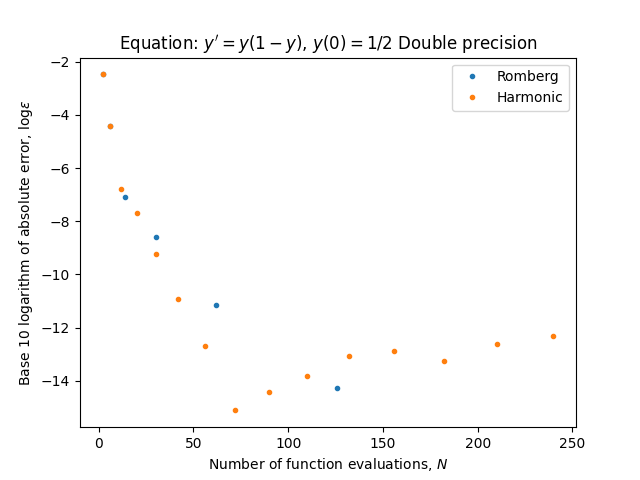
\includegraphics[scale=0.45]{../results/emr_plots/logistic.png}
\end{minipage}
\begin{minipage}{0.45\textwidth}
\centering
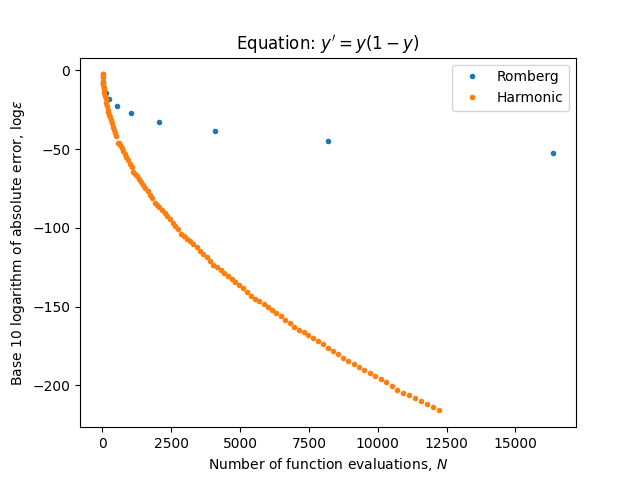
\includegraphics[scale=0.45]{../results/emr_plots/logistic_hp.png}
\end{minipage}
\end{figure}

\begin{figure}[H]
\centering
\begin{minipage}{0.45\textwidth}
\centering
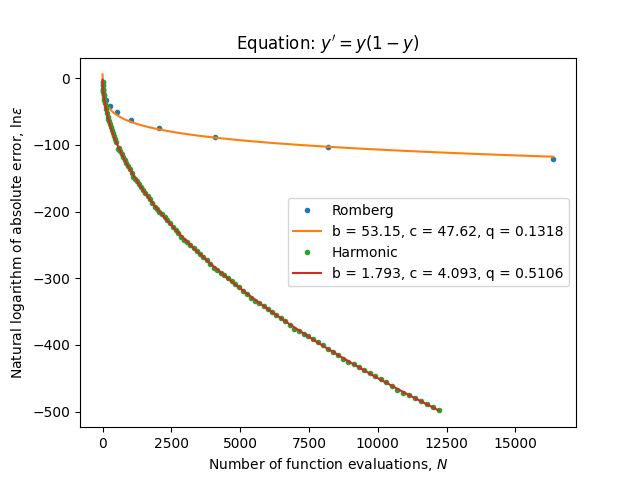
\includegraphics[scale=0.45]{../results/emr_plots/logistic_hp_trend.png}
\end{minipage}
\begin{minipage}{0.45\textwidth}
\centering
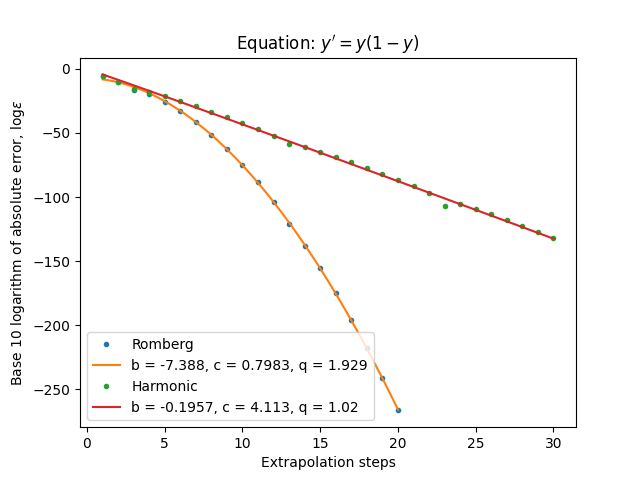
\includegraphics[scale=0.45]{../results/emr_plots/logistic_hp_steps.png}
\end{minipage}
\end{figure}

\begin{figure}[H]
\centering
\begin{minipage}{0.45\textwidth}
\centering
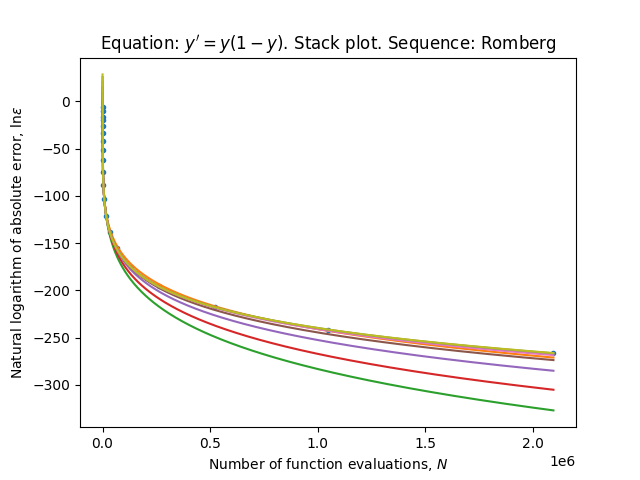
\includegraphics[scale=0.45]{../results/emr_plots/logistic_hp_romberg_stack.png}
\end{minipage}
\begin{minipage}{0.45\textwidth}
\centering
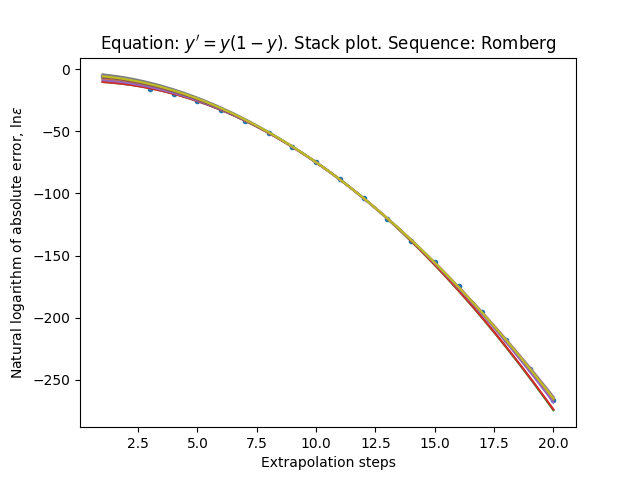
\includegraphics[scale=0.45]{../results/emr_plots/logistic_hp_romberg_steps_stack.png}
\end{minipage}
\end{figure}

\begin{figure}[H]
\centering
\begin{minipage}{0.45\textwidth}
\centering
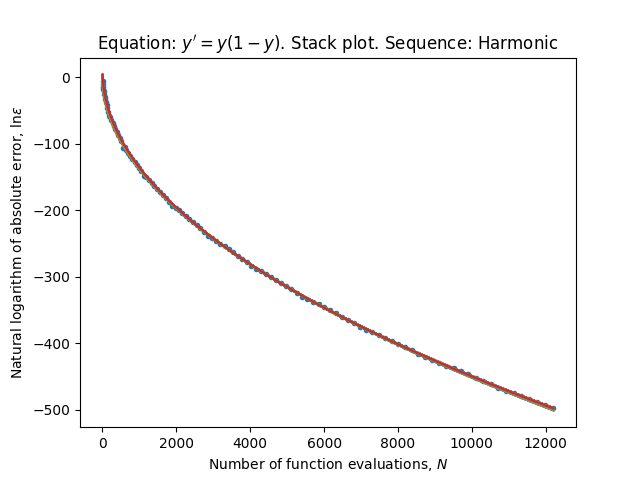
\includegraphics[scale=0.45]{../results/emr_plots/logistic_hp_harmonic_stack.png}
\end{minipage}
\begin{minipage}{0.45\textwidth}
\centering
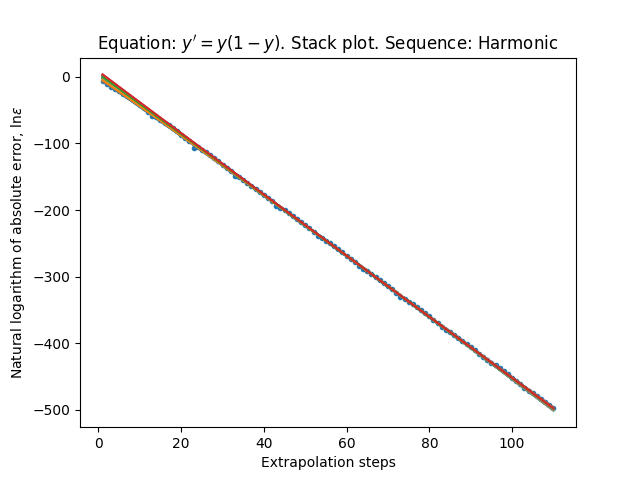
\includegraphics[scale=0.45]{../results/emr_plots/logistic_hp_harmonic_steps_stack.png}
\end{minipage}
\end{figure}

\begin{table}[H]
    \centering
    \small
     \begin{tabular}{c|c||c|c|c|c|c|c}
Sequence & Plot & \(A\)-mean & \(A\)-var & \(c\)-mean & \(c\)-var & \(q\)-mean & \(q\)-var\\\hline
\rowcolor{red}
Romberg & lin-ln evals-error & \(8.848\cdot 10^{63}\) & \(6\) & \(70.69\) & \(0.1952\) & \(0.1226\) & \(0.0637\) \\
\rowcolor{green}
Harmonic & lin-ln evals-error & \(2510\) & \(9.384\) & \(4.249\) & \(0.00357\) & \(0.5073\) & \(0.0001329\) \\
\rowcolor{green}
Romberg & lin-ln steps-error & \(0.01026\) & \(1.856\) & \(0.814\) & \(0.03122\) & \(1.932\) & \(0.001091\) \\
\rowcolor{green}
Harmonic & lin-ln steps-error & \(257.8\) & \(9.223\) & \(4.256\) & \(0.003464\) & \(1.014\) & \(0.0001294\) \\
    \end{tabular}
    \label{tab:my_label}
\end{table}

The harmonic sequence performes better and we get down to machine level precisision using either sequence, in double precision.\\

We seem to have exponential convergence in the number of steps for the Romberg sequence and the models fit well for the harmonic sequence.\\

\subsection{Tangens}

Now we will consider the following equation
\begin{equation}
y'(x) = 1 + y(x)^2, \quad y(0) = 0,\quad x\in [0,1]
\end{equation}

whose solution is 
\[
y(x) \coloneqq \tan(x)
\]
which is meromorphic and we are quite far from singularites.

\begin{figure}[H]
\centering
\begin{minipage}{0.45\textwidth}
\centering
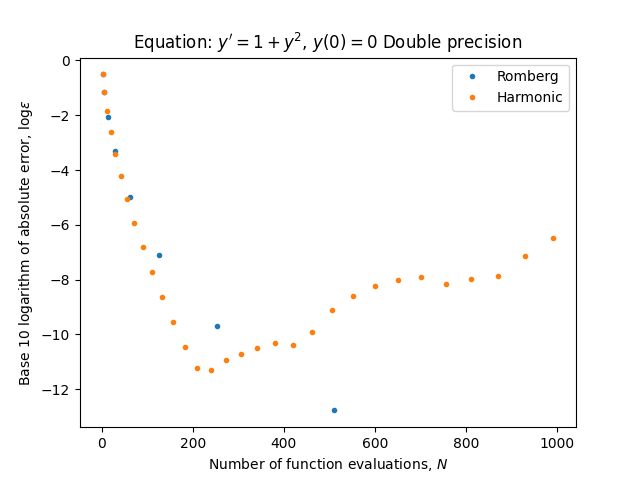
\includegraphics[scale=0.45]{../results/emr_plots/tangens.png}
\end{minipage}
\begin{minipage}{0.45\textwidth}
\centering
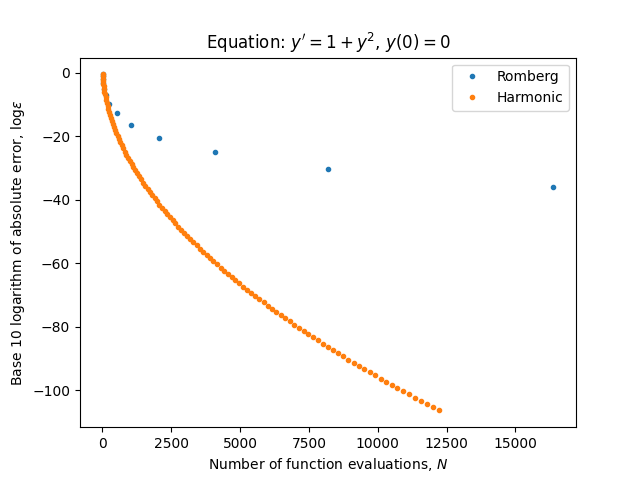
\includegraphics[scale=0.45]{../results/emr_plots/tangens_hp.png}
\end{minipage}
\end{figure}

\begin{figure}[H]
\centering
\begin{minipage}{0.45\textwidth}
\centering
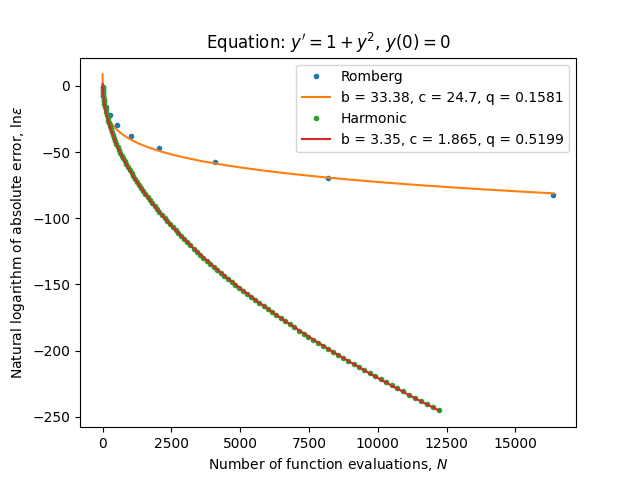
\includegraphics[scale=0.45]{../results/emr_plots/tangens_hp_trend.png}
\end{minipage}
\begin{minipage}{0.45\textwidth}
\centering
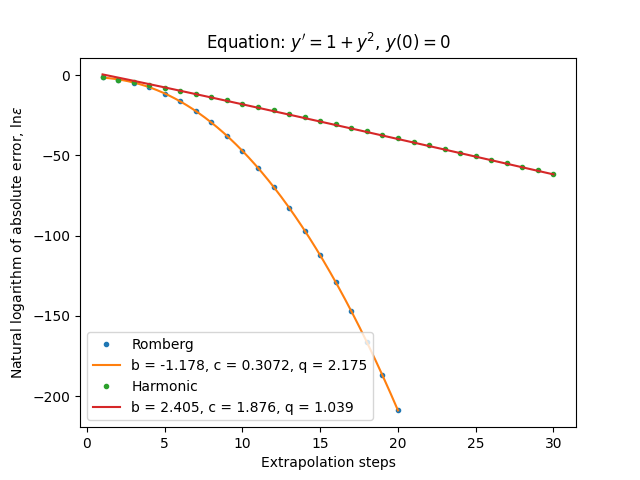
\includegraphics[scale=0.45]{../results/emr_plots/tangens_hp_steps.png}
\end{minipage}
\end{figure}

\begin{figure}[H]
\centering
\begin{minipage}{0.45\textwidth}
\centering
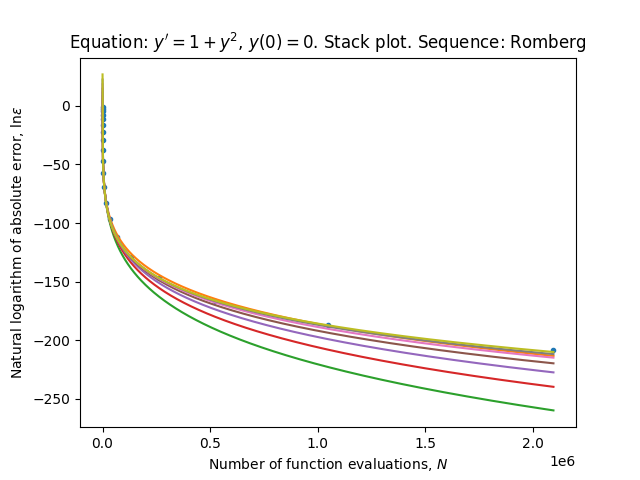
\includegraphics[scale=0.45]{../results/emr_plots/tangens_hp_romberg_stack.png}
\end{minipage}
\begin{minipage}{0.45\textwidth}
\centering
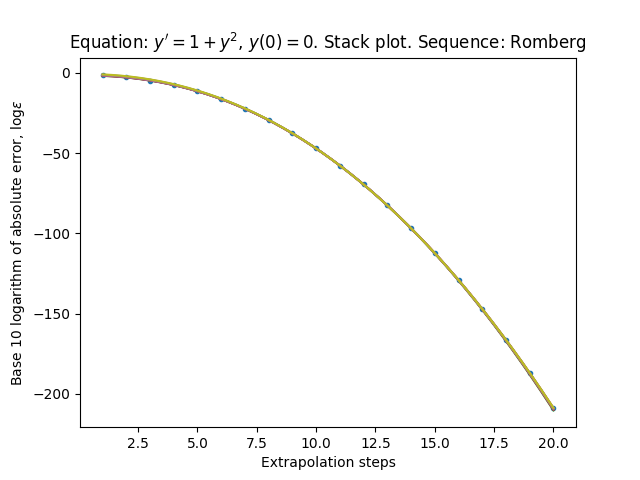
\includegraphics[scale=0.45]{../results/emr_plots/tangens_hp_romberg_steps_stack.png}
\end{minipage}
\end{figure}

\begin{figure}[H]
\centering
\begin{minipage}{0.45\textwidth}
\centering
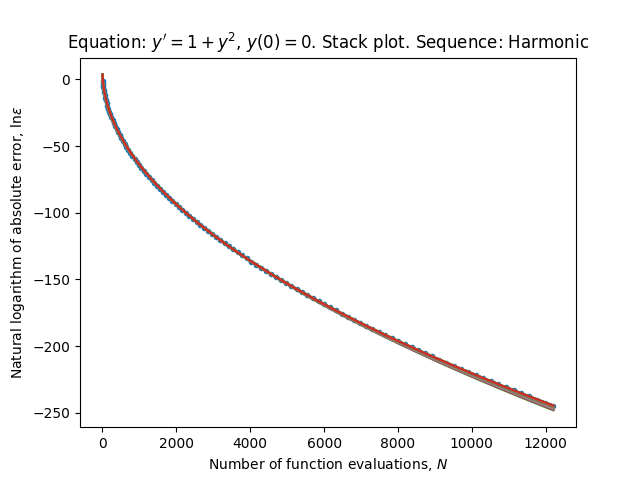
\includegraphics[scale=0.45]{../results/emr_plots/tangens_hp_harmonic_stack.png}
\end{minipage}
\begin{minipage}{0.45\textwidth}
\centering
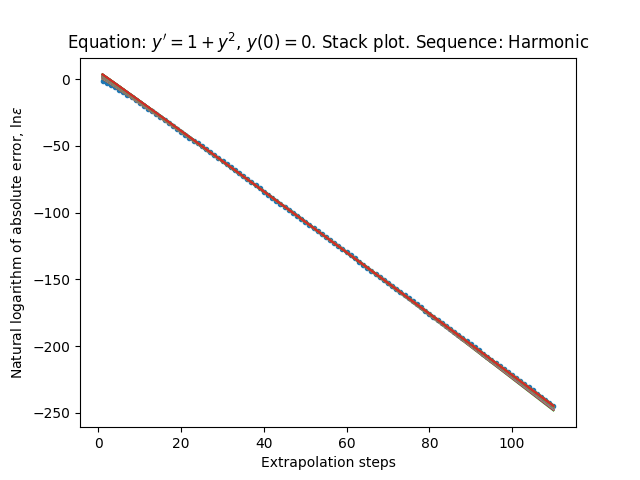
\includegraphics[scale=0.45]{../results/emr_plots/tangens_hp_harmonic_steps_stack.png}
\end{minipage}
\end{figure}

\begin{table}[H]
    \centering
    \small
     \begin{tabular}{c|c||c|c|c|c|c|c}
Sequence & Plot & \(A\)-mean & \(A\)-var & \(c\)-mean & \(c\)-var & \(q\)-mean & \(q\)-var\\\hline
\rowcolor{red}
Romberg & lin-ln evals-error & \(9.496\cdot 10^{36}\) & \(6\) & \(33.25\) & \(0.1689\) & \(0.1523\) & \(0.03648\) \\
\rowcolor{green}
Harmonic & lin-ln evals-error & \(358.8\) & \(0.5652\) & \(2.017\) & \(0.002488\) & \(0.5127\) & \(0.000109\) \\
\rowcolor{green}
Romberg & lin-ln steps-error & \(0.3476\) & \(0.1097\) & \(0.3039\) & \(0.001043\) & \(2.18\) & \(2.579\cdot 10^{-5}\) \\
\rowcolor{green}
Harmonic & lin-ln steps-error & \(121.5\) & \(0.5373\) & \(2.021\) & \(0.002309\) & \(1.025\) & \(0.0001013\) \\
    \end{tabular}
    \label{tab:my_label}
\end{table}

The harmonic sequence performes better and we get down to machine level precision in double precision arithmetic, using either sequence.\\

Here we clearly have exponential convergence in the number of steps for the Romberg sequence and the fit is also very nice for the harmonic sequence.

\subsection{Equation with singularity}

Now we will consider the following initial value problem:
\begin{equation}\label{46}
y'(t) = y^2(t),\quad y(0) = 1/(1+a), \quad t\in [0,1]
\end{equation}

whose solution is 
\[
y(t) = \frac{1}{1-(t-a)}.
\]
The solution is meromorphic with a pole at \(1+a\).

\begin{figure}[H]
\centering
\begin{minipage}{0.45\textwidth}
\centering
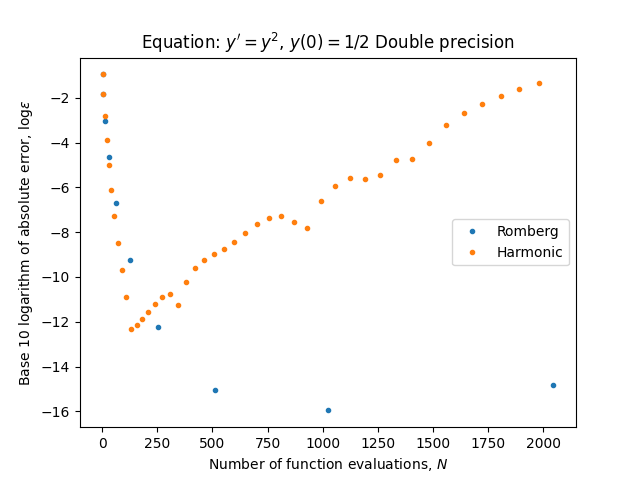
\includegraphics[scale=0.45]{../results/emr_plots/singularity_0.png}
\end{minipage}
\begin{minipage}{0.45\textwidth}
\centering
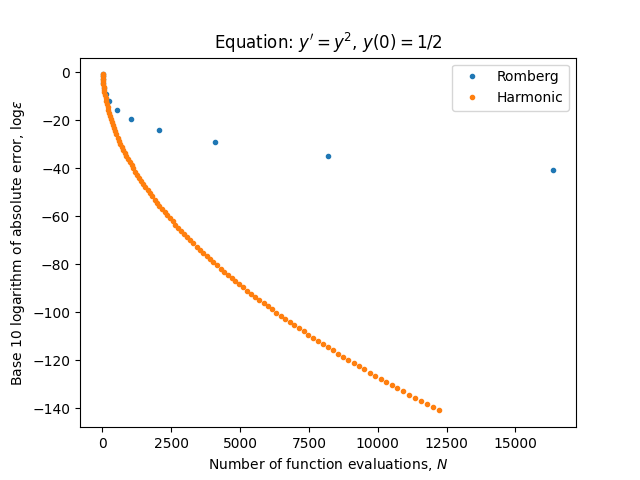
\includegraphics[scale=0.45]{../results/emr_plots/singularity_0_hp.png}
\end{minipage}
\end{figure}

\begin{figure}[H]
\centering
\begin{minipage}{0.45\textwidth}
\centering
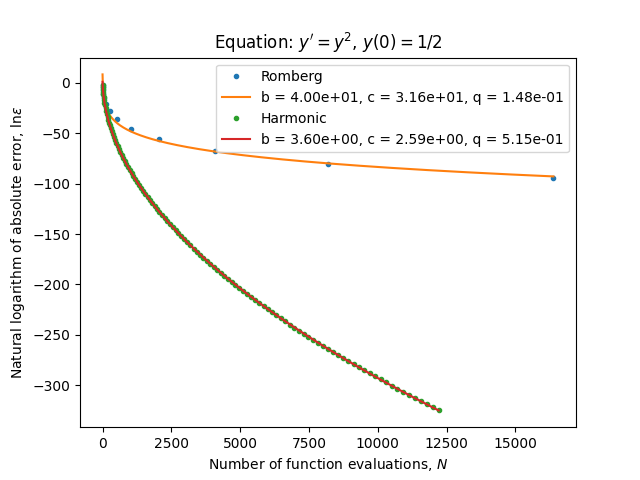
\includegraphics[scale=0.45]{../results/emr_plots/singularity_0_hp_trend.png}
\end{minipage}
\begin{minipage}{0.45\textwidth}
\centering
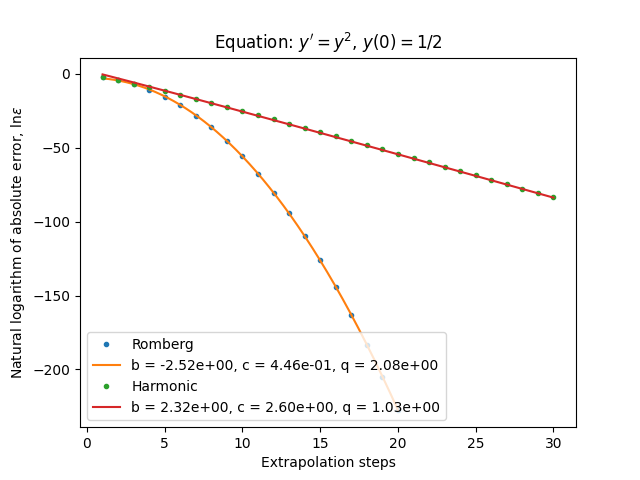
\includegraphics[scale=0.45]{../results/emr_plots/singularity_0_hp_steps.png}
\end{minipage}
\end{figure}

\begin{figure}[H]
\centering
\begin{minipage}{0.45\textwidth}
\centering
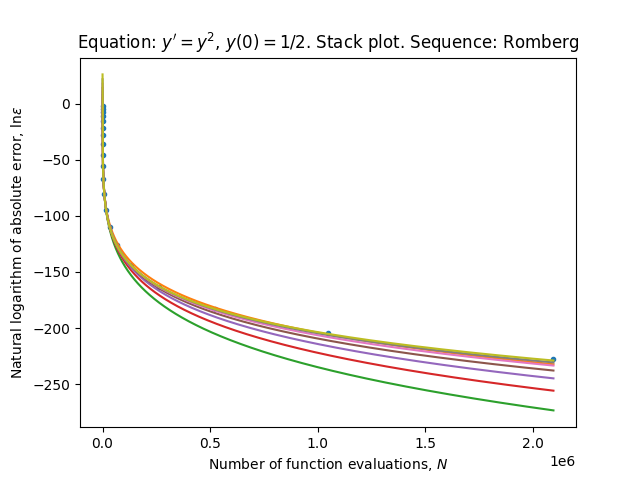
\includegraphics[scale=0.45]{../results/emr_plots/singularity_0_hp_romberg_stack.png}
\end{minipage}
\begin{minipage}{0.45\textwidth}
\centering
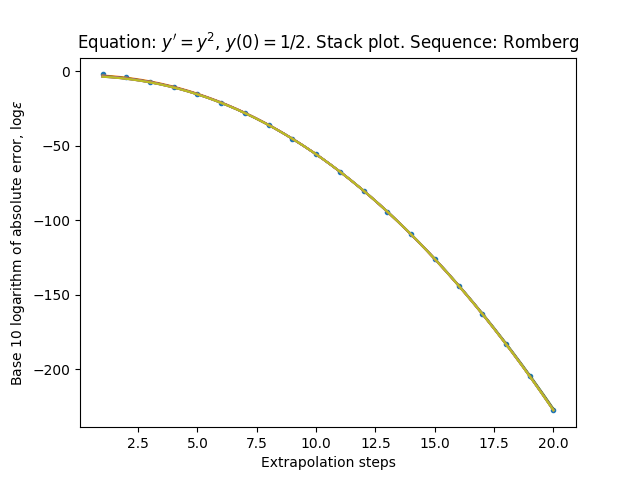
\includegraphics[scale=0.45]{../results/emr_plots/singularity_0_hp_romberg_steps_stack.png}
\end{minipage}
\end{figure}

\begin{figure}[H]
\centering
\begin{minipage}{0.45\textwidth}
\centering
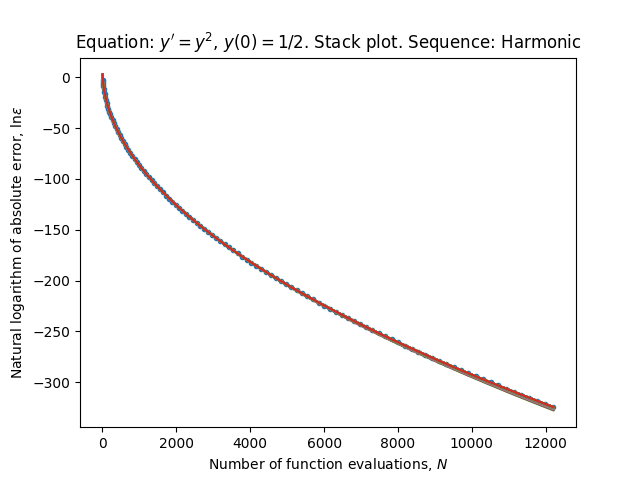
\includegraphics[scale=0.45]{../results/emr_plots/singularity_0_hp_harmonic_stack.png}
\end{minipage}
\begin{minipage}{0.45\textwidth}
\centering
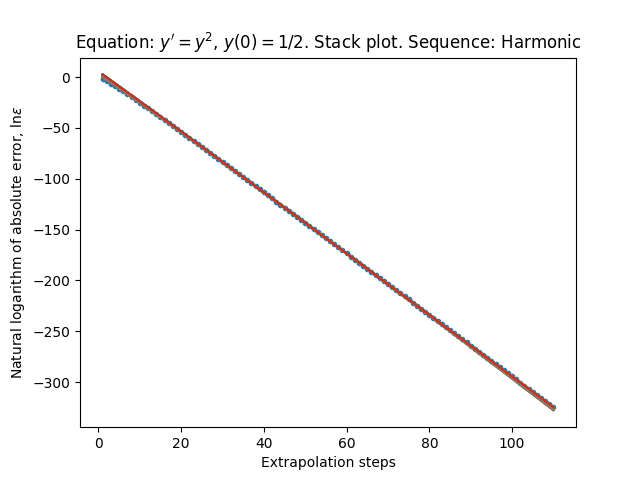
\includegraphics[scale=0.45]{../results/emr_plots/singularity_0_hp_harmonic_steps_stack.png}
\end{minipage}
\end{figure}

\begin{table}[H]
    \centering
    \small
     \begin{tabular}{c|c||c|c|c|c|c|c}
Sequence & Plot & \(A\)-mean & \(A\)-var & \(c\)-mean & \(c\)-var & \(q\)-mean & \(q\)-var\\\hline
\rowcolor{red}
Romberg & lin-ln evals-error & \(1.418\cdot 10^{42}\) & \(6\) & \(42.1\) & \(0.1387\) & \(0.141\) & \(0.03195\) \\
\rowcolor{green}}
Harmonic & lin-ln evals-error & \(440\) & \(0.5196\) & \(2.747\) & \(0.001256\) & \(0.5092\) & \(5.472\cdot 10^{-5}\) \\
\rowcolor{green}
Romberg & lin-ln steps-error & \(0.04186\) & \(0.03016\) & \(0.4274\) & \(0.0002961\) & \(2.091\) & \(8.21\cdot 10^{-6}\) \\
\rowcolor{green}
Harmonic & lin-ln steps-error & \(104.3\) & \(0.4903\) & \(2.752\) & \(0.001151\) & \(1.018\) & \(5.022\cdot 10^{-5}\) \\
    \end{tabular}
    \label{tab:my_label}
\end{table}

The harmonic sequence performes better and we get almost down to machine level precision using standar double precision floating point arithmetic, with either sequence.\\

We have very nice fit for the exponential convergence in the number of steps for the Romberg sequence and also for the harmonic sequence.

\begin{figure}[H]
\centering
\begin{minipage}{0.45\textwidth}
\centering
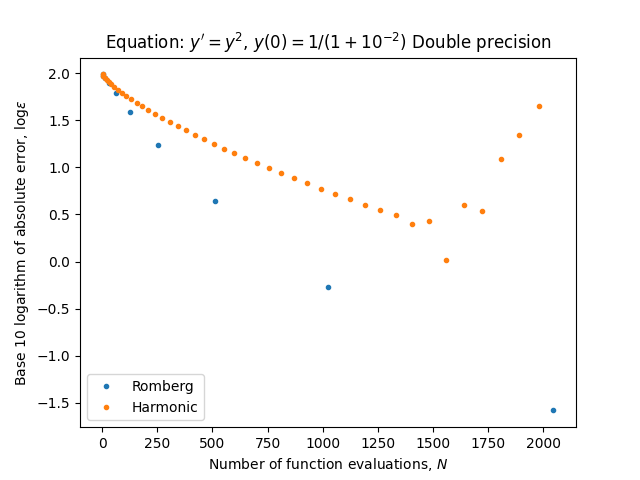
\includegraphics[scale=0.45]{../results/emr_plots/singularity_2.png}
\end{minipage}
\begin{minipage}{0.45\textwidth}
\centering
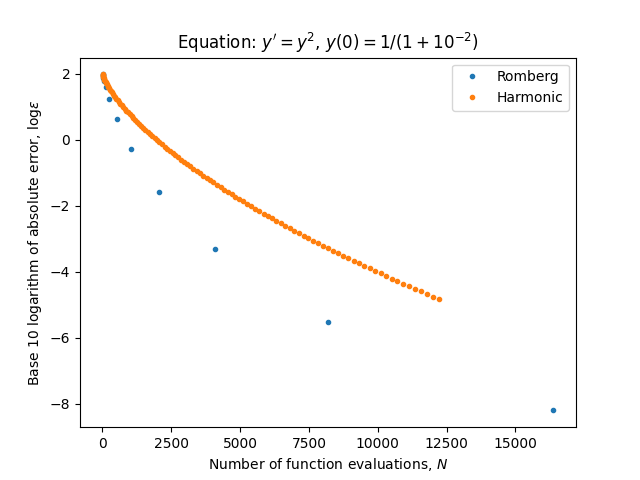
\includegraphics[scale=0.45]{../results/emr_plots/singularity_2_hp.png}
\end{minipage}
\end{figure}

\begin{figure}[H]
\centering
\begin{minipage}{0.45\textwidth}
\centering
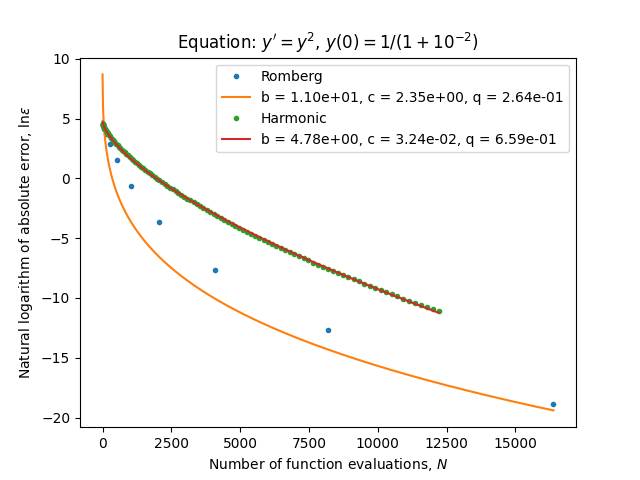
\includegraphics[scale=0.45]{../results/emr_plots/singularity_2_hp_trend.png}
\end{minipage}
\begin{minipage}{0.45\textwidth}
\centering
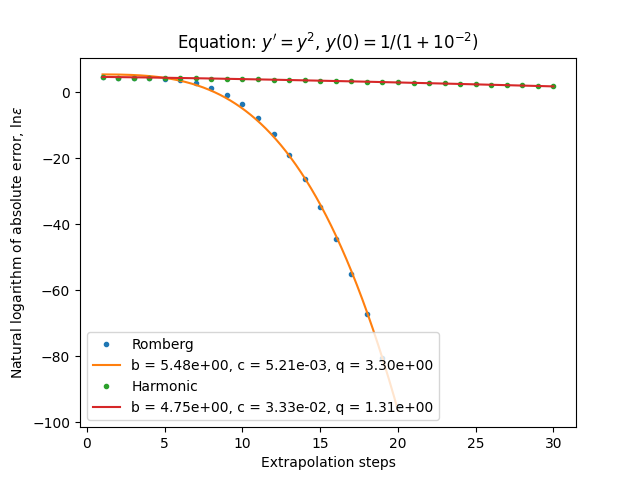
\includegraphics[scale=0.45]{../results/emr_plots/singularity_2_hp_steps.png}
\end{minipage}
\end{figure}

\begin{figure}[H]
\centering
\begin{minipage}{0.45\textwidth}
\centering
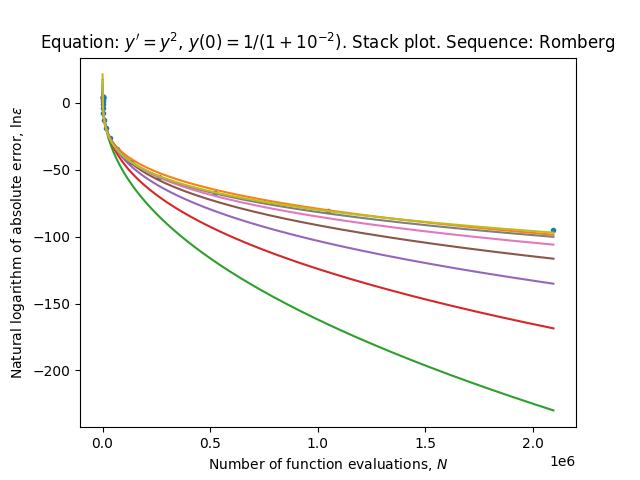
\includegraphics[scale=0.45]{../results/emr_plots/singularity_2_hp_romberg_stack.png}
\end{minipage}
\begin{minipage}{0.45\textwidth}
\centering
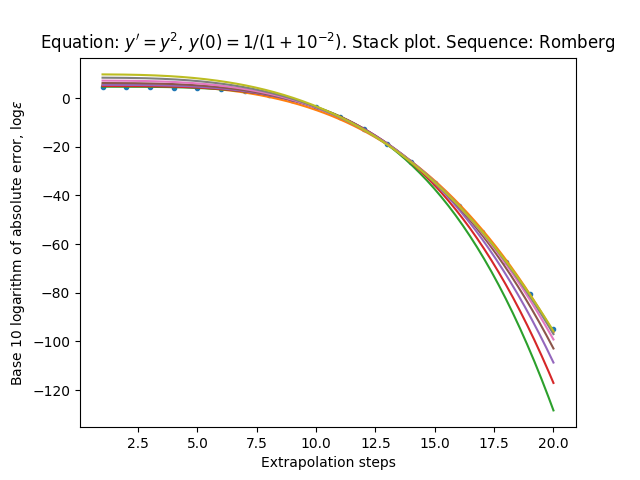
\includegraphics[scale=0.45]{../results/emr_plots/singularity_2_hp_romberg_steps_stack.png}
\end{minipage}
\end{figure}

\begin{figure}[H]
\centering
\begin{minipage}{0.45\textwidth}
\centering
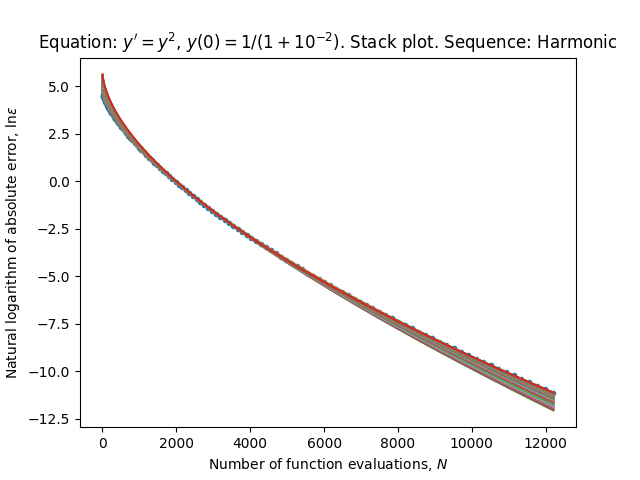
\includegraphics[scale=0.45]{../results/emr_plots/singularity_2_hp_harmonic_stack.png}
\end{minipage}
\begin{minipage}{0.45\textwidth}
\centering
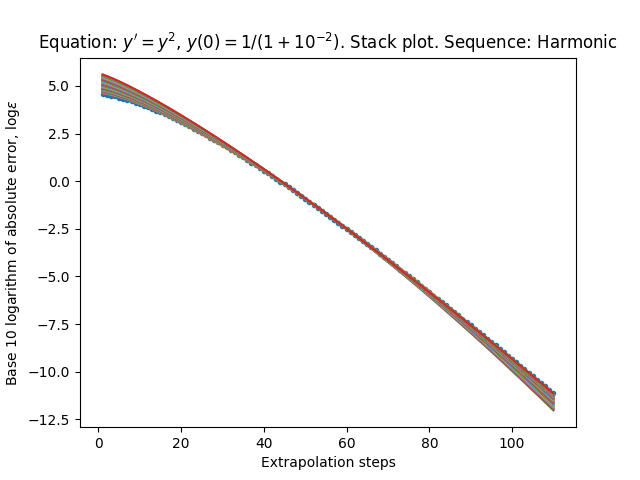
\includegraphics[scale=0.45]{../results/emr_plots/singularity_2_hp_harmonic_steps_stack.png}
\end{minipage}
\end{figure}

\begin{table}[H]
    \centering
    \small
     \begin{tabular}{c|c||c|c|c|c|c|c}
Sequence & Plot & \(A\)-mean & \(A\)-var & \(c\)-mean & \(c\)-var & \(q\)-mean & \(q\)-var\\\hline
\rowcolor{red}
Romberg & lin-ln evals-error & \(1.249\cdot 10^{12}\) & \(5.984\) & \(2.77\) & \(0.7656\) & \(0.3067\) & \(0.08315\) \\
\rowcolor{green}
Harmonic & lin-ln evals-error & \(173.2\) & \(0.1158\) & \(0.03983\) & \(0.08603\) & \(0.6452\) & \(0.002375\) \\
\rowcolor{green}
Romberg & lin-ln steps-error & \(3540\) & \(2.885\) & \(0.005212\) & \(0.6307\) & \(3.461\) & \(0.00941\) \\
\rowcolor{green}
Harmonic & lin-ln steps-error & \(165.2\) & \(0.1095\) & \(0.04047\) & \(0.08154\) & \(1.287\) & \(0.002248\) \\
    \end{tabular}
    \label{tab:my_label}
\end{table}

Here Romberg works better and we do not attain as high precisison using the harmonic as when using Romberg, in standard double precision arithmetic.\\

Here the model fits moderately well for Romberg sequence, when considering exponential convergence in the number of steps. We also have moderate fit for the harmonic sequence.

\begin{figure}[H]
\centering
\begin{minipage}{0.45\textwidth}
\centering
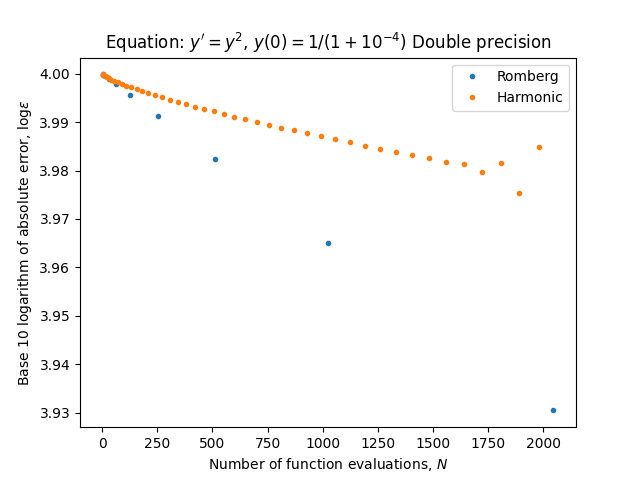
\includegraphics[scale=0.45]{../results/emr_plots/singularity_4.png}
\end{minipage}
\begin{minipage}{0.45\textwidth}
\centering
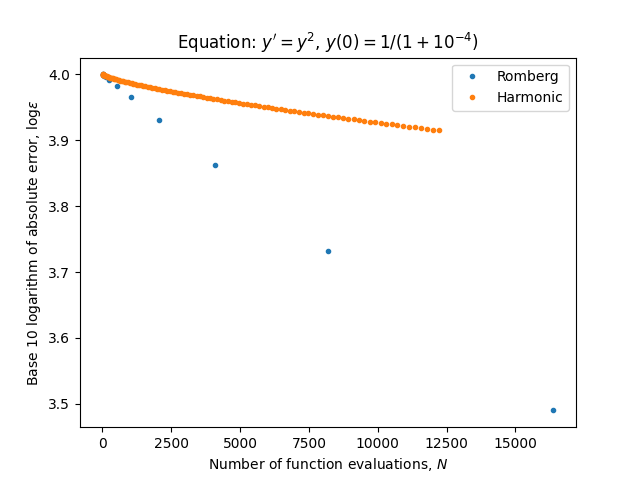
\includegraphics[scale=0.45]{../results/emr_plots/singularity_4_hp.png}
\end{minipage}
\end{figure}

\begin{figure}[H]
\centering
\begin{minipage}{0.45\textwidth}
\centering
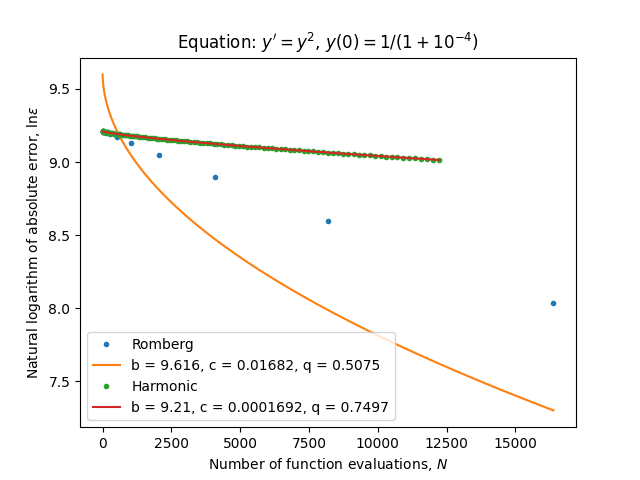
\includegraphics[scale=0.45]{../results/emr_plots/singularity_4_hp_trend.png}
\end{minipage}
\begin{minipage}{0.45\textwidth}
\centering
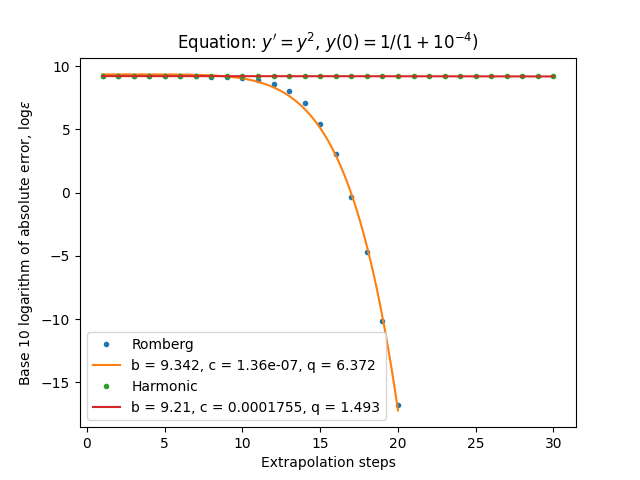
\includegraphics[scale=0.45]{../results/emr_plots/singularity_4_hp_steps.png}
\end{minipage}
\end{figure}

\begin{figure}[H]
\centering
\begin{minipage}{0.45\textwidth}
\centering
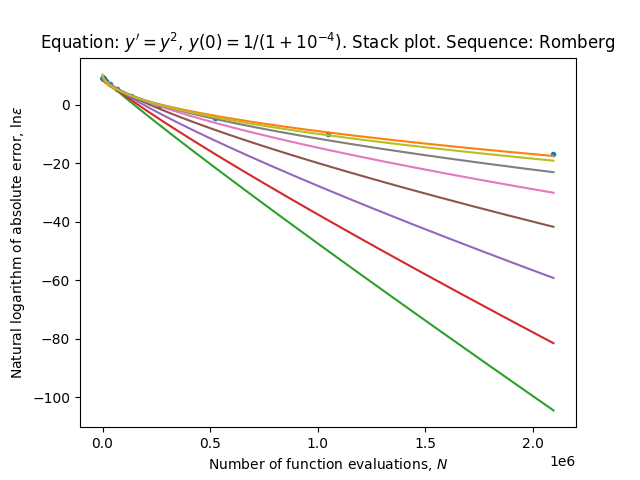
\includegraphics[scale=0.45]{../results/emr_plots/singularity_4_hp_romberg_stack.png}
\end{minipage}
\begin{minipage}{0.45\textwidth}
\centering
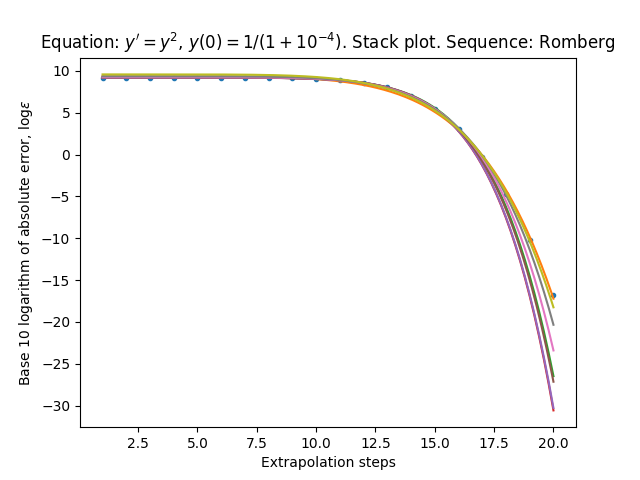
\includegraphics[scale=0.45]{../results/emr_plots/singularity_4_hp_romberg_steps_stack.png}
\end{minipage}
\end{figure}

\begin{figure}[H]
\centering
\begin{minipage}{0.45\textwidth}
\centering
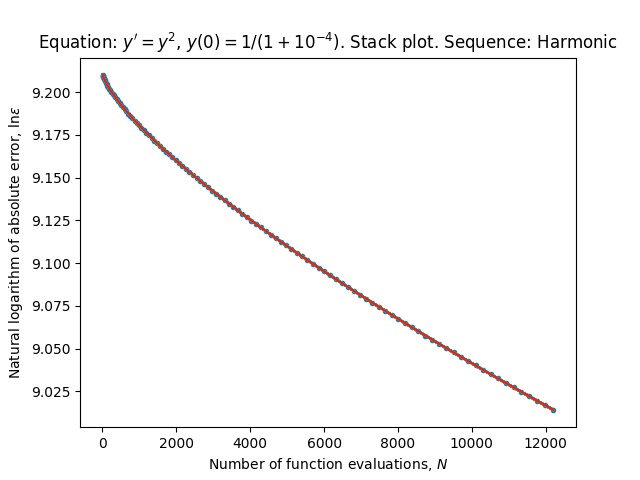
\includegraphics[scale=0.45]{../results/emr_plots/singularity_4_hp_harmonic_stack.png}
\end{minipage}
\begin{minipage}{0.45\textwidth}
\centering
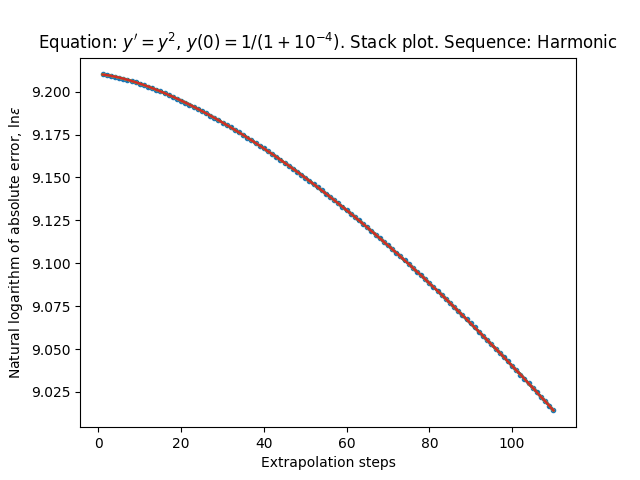
\includegraphics[scale=0.45]{../results/emr_plots/singularity_4_hp_harmonic_steps_stack.png}
\end{minipage}
\end{figure}


\begin{table}[H]
    \centering
    \small
     \begin{tabular}{c|c||c|c|c|c|c|c}
Sequence & Plot & \(A\)-mean & \(A\)-var & \(c\)-mean & \(c\)-var & \(q\)-mean & \(q\)-var\\\hline
\rowcolor{red}
Romberg & lin-ln evals-error & \(1.462\cdot 10^4\) & \(0.2298\) & \(0.004335\) & \(2.285\) & \(0.7393\) & \(0.04196\) \\
\rowcolor{yellow}
Harmonic & lin-ln evals-error & \(1\cdot 10^4\) & \(5.52\cdot 10^{-9}\) & \(0.0001699\) & \(5.806\cdot 10^{-5}\) & \(0.7494\) & \(1.194\cdot 10^{-6}\) \\
\rowcolor{yellow}
Romberg & lin-ln steps-error & \(1.087\cdot 10^4\) & \(0.02206\) & \(1.977\cdot 10^{-8}\) & \(3.201\) & \(7.604\) & \(0.006289\) \\
\rowcolor{yellow}
Harmonic & lin-ln steps-error & \(9997\) & \(3.302\cdot 10^{-10}\) & \(0.0001749\) & \(5.29\cdot 10^{-6}\) & \(1.494\) & \(1.204\cdot 10^{-7}\) \\
    \end{tabular}
    \label{tab:my_label}
\end{table}

Here we clearly do not have exponential convergence in the number of evaluations for the Romberg sequence. We have not so good fit for exponential convergence in the number of steps.\\

Regarding the harmonic sequence, we note that we have extremely slow convergence, so the \(x\) and \(y\) values differ by many orders of magnitude, so the results are maybe not so reliable.

\subsection{Equation with moderate singularity}

Now we will consider the following initial value problem
\begin{equation}
y'(t) = -\frac{1}{2y}, \quad y(0) = \sqrt{1+a},\quad t\in [0,1]\label{47}
\end{equation}
whose solution is 
\[
y(t) = \sqrt{1 - (t-a)}
\]

\begin{figure}[H]
\centering
\begin{minipage}{0.45\textwidth}
\centering
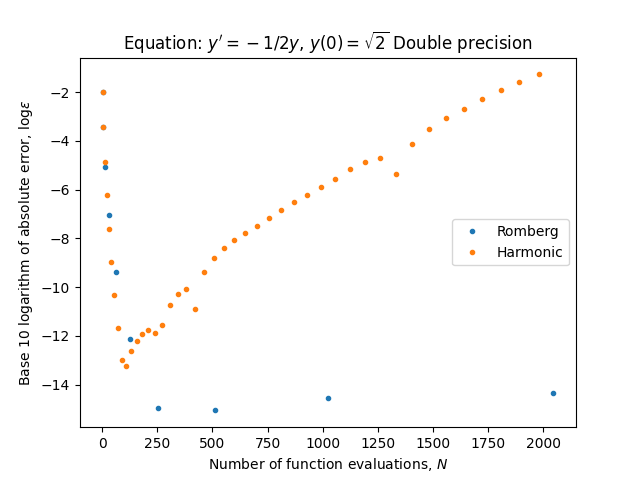
\includegraphics[scale=0.45]{../results/emr_plots/quad_sing_0.png}
\end{minipage}
\begin{minipage}{0.45\textwidth}
\centering
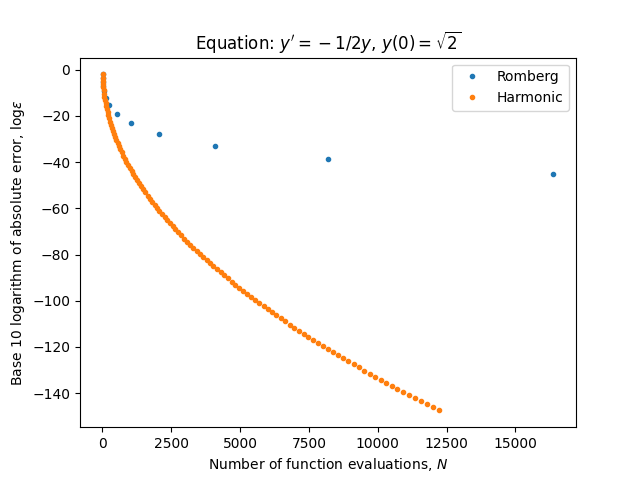
\includegraphics[scale=0.45]{../results/emr_plots/quad_sing_0_hp.png}
\end{minipage}
\end{figure}

\begin{figure}[H]
\centering
\begin{minipage}{0.45\textwidth}
\centering
\includegraphics[scale=0.45]{../results/emr_plots/quad_sing_0_hp_trend.png}
\end{minipage}
\begin{minipage}{0.45\textwidth}
\centering
\includegraphics[scale=0.45]{../results/emr_plots/quad_sing_0_hp_steps.png}
\end{minipage}
\end{figure}

\begin{figure}[H]
\centering
\begin{minipage}{0.45\textwidth}
\centering
\includegraphics[scale=0.45]{../results/emr_plots/quad_sing_0_hp_romberg_stack.png}
\end{minipage}
\begin{minipage}{0.45\textwidth}
\centering
\includegraphics[scale=0.45]{../results/emr_plots/quad_sing_0_hp_romberg_steps_stack.png}
\end{minipage}
\end{figure}

\begin{figure}[H]
\centering
\begin{minipage}{0.45\textwidth}
\centering
\includegraphics[scale=0.45]{../results/emr_plots/quad_sing_0_hp_harmonic_stack.png}
\end{minipage}
\begin{minipage}{0.45\textwidth}
\centering
\includegraphics[scale=0.45]{../results/emr_plots/quad_sing_0_hp_harmonic_steps_stack.png}
\end{minipage}
\end{figure}

\begin{table}[H]
    \centering
    \small
     \begin{tabular}{c|c||c|c|c|c|c|c}
Sequence & Plot & \(A\)-mean & \(A\)-var & \(c\)-mean & \(c\)-var & \(q\)-mean & \(q\)-var\\\hline
\rowcolor{red}
Romberg & lin-ln evals-error & \(8.335\cdot 10^{41}\) & \(6\) & \(47.04\) & \(0.1111\) & \(0.1343\) & \(0.02593\) \\
\rowcolor{green}
Harmonic & lin-ln evals-error & \(0.454\) & \(0.03631\) & \(3.115\) & \(3.797\cdot 10^{-5}\) & \(0.4983\) & \(1.623\cdot 10^{-6}\) \\
\rowcolor{green}
Romberg & lin-ln steps-error & \(0.0002771\) & \(0.7384\) & \(0.5104\) & \(0.0058\) & \(2.038\) & \(0.0001599\) \\
\rowcolor{green}
Harmonic & lin-ln steps-error & \(0.1009\) & \(0.0414\) & \(3.117\) & \(4.412\cdot 10^{-5}\) & \(0.9965\) & \(1.9\cdot 10^{-6}\) \\
    \end{tabular}
    \label{tab:my_label}
\end{table}

Here the harmonic sequence works better than Romberg and we get down to machine level precision using either sequence, in standard double precision floating point arithmetic.\\

Here we clearly have exponential convergence in the number of steps and evaluations for the harmonic sequence. Regarding Romberg, we seem to have exponential convergence in the number of steps.

\begin{figure}[H]
\centering
\begin{minipage}{0.45\textwidth}
\centering
\includegraphics[scale=0.45]{../results/emr_plots/quad_sing_2.png}
\end{minipage}
\begin{minipage}{0.45\textwidth}
\centering
\includegraphics[scale=0.45]{../results/emr_plots/quad_sing_2_hp.png}
\end{minipage}
\end{figure}

\begin{figure}[H]
\centering
\begin{minipage}{0.45\textwidth}
\centering
\includegraphics[scale=0.45]{../results/emr_plots/quad_sing_2_hp_trend.png}
\end{minipage}
\begin{minipage}{0.45\textwidth}
\centering
\includegraphics[scale=0.45]{../results/emr_plots/quad_sing_2_hp_steps.png}
\end{minipage}
\end{figure}

\begin{figure}[H]
\centering
\begin{minipage}{0.45\textwidth}
\centering
\includegraphics[scale=0.45]{../results/emr_plots/quad_sing_2_hp_romberg_stack.png}
\end{minipage}
\begin{minipage}{0.45\textwidth}
\centering
\includegraphics[scale=0.45]{../results/emr_plots/quad_sing_2_hp_romberg_steps_stack.png}
\end{minipage}
\end{figure}

\begin{figure}[H]
\centering
\begin{minipage}{0.45\textwidth}
\centering
\includegraphics[scale=0.45]{../results/emr_plots/quad_sing_2_hp_harmonic_stack.png}
\end{minipage}
\begin{minipage}{0.45\textwidth}
\centering
\includegraphics[scale=0.45]{../results/emr_plots/quad_sing_2_hp_harmonic_steps_stack.png}
\end{minipage}
\end{figure}

\begin{table}[H]
    \centering
    \small
    \begin{tabular}{c|c||c|c|c|c|c|c}
Sequence & Plot & \(A\)-mean & \(A\)-var & \(c\)-mean & \(c\)-var & \(q\)-mean & \(q\)-var\\\hline
\rowcolor{red}
Romberg & lin-ln evals-error & \(3.095\cdot 10^9\) & \(5.978\) & \(4.521\) & \(0.4282\) & \(0.2537\) & \(0.04639\) \\
\rowcolor{green}
Harmonic & lin-ln evals-error & \(0.09273\) & \(0.0545\) & \(0.263\) & \(0.01142\) & \(0.4785\) & \(0.0004549\) \\
\rowcolor{green}
Romberg & lin-ln steps-error & \(0.2097\) & \(1.241\) & \(0.01393\) & \(0.1057\) & \(3.022\) & \(0.001297\) \\
\rowcolor{green}
Harmonic & lin-ln steps-error & \(0.08262\) & \(0.05039\) & \(0.2624\) & \(0.01092\) & \(0.9574\) & \(0.0004388\) \\
    \end{tabular}
    \label{tab:my_label}
\end{table}

Here Romberg performes better and we do not attain as high precision using the harmonic sequence in standard double precision floating point arithmetic.\\

For the Romberg sequence, the model seems to fit moderately well when considering exponential convergence in the number of evaluations. We also have reasonably good fit for the harmonic sequence.\\

\begin{figure}[H]
\centering
\begin{minipage}{0.45\textwidth}
\centering
\includegraphics[scale=0.45]{../results/emr_plots/quad_sing_4.png}
\end{minipage}
\begin{minipage}{0.45\textwidth}
\centering
\includegraphics[scale=0.45]{../results/emr_plots/quad_sing_4_hp.png}
\end{minipage}
\end{figure}

\begin{figure}[H]
\centering
\begin{minipage}{0.45\textwidth}
\centering
\includegraphics[scale=0.45]{../results/emr_plots/quad_sing_4_hp_trend.png}
\end{minipage}
\begin{minipage}{0.45\textwidth}
\centering
\includegraphics[scale=0.45]{../results/emr_plots/quad_sing_4_hp_steps.png}
\end{minipage}
\end{figure}

\begin{figure}[H]
\centering
\begin{minipage}{0.45\textwidth}
\centering
\includegraphics[scale=0.45]{../results/emr_plots/quad_sing_4_hp_romberg_stack.png}
\end{minipage}
\begin{minipage}{0.45\textwidth}
\centering
\includegraphics[scale=0.45]{../results/emr_plots/quad_sing_4_hp_romberg_steps_stack.png}
\end{minipage}
\end{figure}

\begin{figure}[H]
\centering
\begin{minipage}{0.45\textwidth}
\centering
\includegraphics[scale=0.45]{../results/emr_plots/quad_sing_4_hp_harmonic_stack.png}
\end{minipage}
\begin{minipage}{0.45\textwidth}
\centering
\includegraphics[scale=0.45]{../results/emr_plots/quad_sing_4_hp_harmonic_steps_stack.png}
\end{minipage}
\end{figure}

\begin{table}[H]
    \centering
    \small
     \begin{tabular}{c|c||c|c|c|c|c|c}
Sequence & Plot & \(A\)-mean & \(A\)-var & \(c\)-mean & \(c\)-var & \(q\)-mean & \(q\)-var\\\hline
\rowcolor{red}
Romberg & lin-ln evals-error & \(0.1398\) & \(0.4846\) & \(0.2489\) & \(0.4625\) & \(0.3506\) & \(0.01881\) \\
\rowcolor{red}
Harmonic & lin-ln evals-error & \(1.282\) & \(3.403\) & \(1.258\) & \(0.3894\) & \(0.1631\) & \(0.05472\) \\
\rowcolor{red}
Romberg & lin-ln steps-error & \(0.0429\) & \(0.5116\) & \(0.001785\) & \(3.769\) & \(4.002\) & \(0.04408\) \\
\rowcolor{red}
Harmonic & lin-ln steps-error & \(0.8136\) & \(1.714\) & \(1.146\) & \(0.311\) & \(0.3342\) & \(0.04634\) \\
    \end{tabular}
    \label{tab:my_label}
\end{table}

Here, we do not have any clear fit.

\subsection{Circular rotation}

Now we will consider the following system of equations:
\begin{equation}\label{48}
(y_1(t),y_2(t))' = (-y_2(t), y_1(t)), \quad y(0) = (1,0), \quad t\in [0,\pi /2]
\end{equation}
whose solution is 
\[
(y_1(t),y_2(t)) = (\cos t, \sin t)
\]
which is entire.

\begin{figure}[H]
\centering
\begin{minipage}{0.45\textwidth}
\centering
\includegraphics[scale=0.45]{../results/emr_plots/rotation.png}
\end{minipage}
\begin{minipage}{0.45\textwidth}
\centering
\includegraphics[scale=0.45]{../results/emr_plots/rotation_hp.png}
\end{minipage}
\end{figure}

\begin{figure}[H]
\centering
\begin{minipage}{0.45\textwidth}
\centering
\includegraphics[scale=0.45]{../results/emr_plots/rotation_hp_trend.png}
\end{minipage}
\begin{minipage}{0.45\textwidth}
\centering
\includegraphics[scale=0.45]{../results/emr_plots/rotation_hp_steps.png}
\end{minipage}
\end{figure}

\begin{figure}[H]
\centering
\begin{minipage}{0.45\textwidth}
\centering
\includegraphics[scale=0.45]{../results/emr_plots/rotation_hp_romberg_stack.png}
\end{minipage}
\begin{minipage}{0.45\textwidth}
\centering
\includegraphics[scale=0.45]{../results/emr_plots/rotation_hp_romberg_steps_stack.png}
\end{minipage}
\end{figure}

\begin{figure}[H]
\centering
\begin{minipage}{0.45\textwidth}
\centering
\includegraphics[scale=0.45]{../results/emr_plots/rotation_hp_harmonic_stack.png}
\end{minipage}
\begin{minipage}{0.45\textwidth}
\centering
\includegraphics[scale=0.45]{../results/emr_plots/rotation_hp_harmonic_steps_stack.png}
\end{minipage}
\end{figure}

\begin{table}[H]
    \centering
    \small
     \begin{tabular}{c|c||c|c|c|c|c|c}
Sequence & Plot & \(A\)-mean & \(A\)-var & \(c\)-mean & \(c\)-var & \(q\)-mean & \(q\)-var\\\hline
\rowcolor{red}
Romberg & lin-ln evals-error & \(1.215\cdot 10^{60}\) & \(6\) & \(61.05\) & \(0.1358\) & \(0.1308\) & \(0.03453\) \\
\rowcolor{yellow}
Harmonic & lin-ln evals-error & \(9\cdot 10^9\) & \(6.841\) & \(2.636\) & \(0.007896\) & \(0.62\) & \(0.0002457\) \\
\rowcolor{green}
Romberg & lin-ln steps-error & \(1.083\) & \(0.000101\) & \(0.6717\) & \(4.963\cdot 10^{-7}\) & \(2.007\) & \(1.48\cdot 10^{-8}\) \\
\rowcolor{yellow}
Harmonic & lin-ln steps-error & \(4.276\cdot 10^8\) & \(6.508\) & \(2.675\) & \(0.006923\) & \(1.237\) & \(0.0002153\) \\
    \end{tabular}
    \label{tab:my_label}
\end{table}

The harmonic sequence works better then Romberg and we get down to machine level precision using either sequence when using standard floating point arithmetic.\\

We clearly have exponential convergence in the number of steps for the Romberg sequence. For the harmonic sequence, we seem to have exponential convergence, but though we must note that the mean value of the \(A\) coefficient is suspiciously large.

\subsection{Mathematical pendulum}

Now we will consider the mathematical pendulum equation:
\begin{equation}
y''(t) + \sin y(t) = 0,\quad y(0) = 0,\, y'(0) = 1, \quad t\in [0,1].
\end{equation}

\begin{figure}[H]
\centering
\begin{minipage}{0.45\textwidth}
\centering
\includegraphics[scale=0.45]{../results/emr_plots/oscillation.png}
\end{minipage}
\begin{minipage}{0.45\textwidth}
\centering
\includegraphics[scale=0.45]{../results/emr_plots/oscillation_hp.png}
\end{minipage}
\end{figure}

\begin{figure}[H]
\centering
\begin{minipage}{0.45\textwidth}
\centering
\includegraphics[scale=0.45]{../results/emr_plots/oscillation_hp_trend.png}
\end{minipage}
\begin{minipage}{0.45\textwidth}
\centering
\includegraphics[scale=0.45]{../results/emr_plots/oscillation_hp_steps.png}
\end{minipage}
\end{figure}

\begin{figure}[H]
\centering
\begin{minipage}{0.45\textwidth}
\centering
\includegraphics[scale=0.45]{../results/emr_plots/oscillation_hp_romberg_stack.png}
\end{minipage}
\begin{minipage}{0.45\textwidth}
\centering
\includegraphics[scale=0.45]{../results/emr_plots/oscillation_hp_romberg_steps_stack.png}
\end{minipage}
\end{figure}

\begin{figure}[H]
\centering
\begin{minipage}{0.45\textwidth}
\centering
\includegraphics[scale=0.45]{../results/emr_plots/oscillation_hp_harmonic_stack.png}
\end{minipage}
\begin{minipage}{0.45\textwidth}
\centering
\includegraphics[scale=0.45]{../results/emr_plots/oscillation_hp_harmonic_steps_stack.png}
\end{minipage}
\end{figure}

\begin{table}[H]
    \centering
    \small
     \begin{tabular}{c|c||c|c|c|c|c|c}
Sequence & Plot & \(A\)-mean & \(A\)-var & \(c\)-mean & \(c\)-var & \(q\)-mean & \(q\)-var\\\hline
\rowcolor{red}
Romberg & lin-ln evals-error & \(3.245\cdot 10^{52}\) & \(6\) & \(56.9\) & \(0.1423\) & \(0.1295\) & \(0.03859\) \\
\rowcolor{green}
Harmonic & lin-ln evals-error & \(471.5\) & \(0.2744\) & \(3.713\) & \(0.0002618\) & \(0.5042\) & \(1.13\cdot 10^{-5}\) \\
\rowcolor{green}
Romberg & lin-ln steps-error & \(0.01384\) & \(0.3333\) & \(0.6305\) & \(0.002076\) & \(1.995\) & \(6.207\cdot 10^{-5}\) \\
\rowcolor{green}
Harmonic & lin-ln steps-error & \(72.54\) & \(0.2499\) & \(3.718\) & \(0.0002297\) & \(1.008\) & \(9.918\cdot 10^{-6}\) \\
    \end{tabular}
    \label{tab:my_label}
\end{table}

Here the harmonic sequence works better and we get down to machine level precision in standard double precision floating point arithmetic, using either sequence.\\

We have nice fit for the exponential convergence in the number of steps for the Romberg sequence. We also have very nice fit for the harmonic sequence.

\subsection{Federpendel}

Now we will consider the equation of motion for das Federpendel or the spring pendulum:
\[
\bfp' = -(|\bfq| - 1)\frac{\bfq}{|\bfq|} - {1\choose 0}, \quad \bfq' = \bfp
\]
where \(\bfp\) and \(\bfq\) are two dimensional vectors. We will consider it with the initial condition \(\bfq(0) = (1,0)\) and \(\bfp(0) = (0,1)\) and try to both estimate the solution at time \(t = 1\) and time \(t = 2\).

\begin{figure}[H]
\centering
\begin{minipage}{0.45\textwidth}
\centering
\includegraphics[scale=0.45]{../results/emr_plots/federpendel.png}
\end{minipage}
\begin{minipage}{0.45\textwidth}
\centering
\includegraphics[scale=0.45]{../results/emr_plots/federpendel_1_hp.png}
\end{minipage}
\end{figure}

\begin{figure}[H]
\centering
\begin{minipage}{0.45\textwidth}
\centering
\includegraphics[scale=0.45]{../results/emr_plots/federpendel_1_hp_trend.png}
\end{minipage}
\begin{minipage}{0.45\textwidth}
\centering
\includegraphics[scale=0.45]{../results/emr_plots/federpendel_1_hp_steps.png}
\end{minipage}
\end{figure}

\begin{figure}[H]
\centering
\begin{minipage}{0.45\textwidth}
\centering
\includegraphics[scale=0.45]{../results/emr_plots/federpendel_1_hp_romberg_stack.png}
\end{minipage}
\begin{minipage}{0.45\textwidth}
\centering
\includegraphics[scale=0.45]{../results/emr_plots/federpendel_1_hp_romberg_steps_stack.png}
\end{minipage}
\end{figure}

\begin{figure}[H]
\centering
\begin{minipage}{0.45\textwidth}
\centering
\includegraphics[scale=0.45]{../results/emr_plots/federpendel_1_hp_harmonic_stack.png}
\end{minipage}
\begin{minipage}{0.45\textwidth}
\centering
\includegraphics[scale=0.45]{../results/emr_plots/federpendel_1_hp_harmonic_steps_stack.png}
\end{minipage}
\end{figure}

\begin{table}[H]
    \centering
    \small
     \begin{tabular}{c|c||c|c|c|c|c|c}
Sequence & Plot & \(A\)-mean & \(A\)-var & \(c\)-mean & \(c\)-var & \(q\)-mean & \(q\)-var\\\hline
\rowcolor{red}
Romberg & lin-ln evals-error & \(8.241\cdot 10^{40}\) & \(6\) & \(43.86\) & \(0.1208\) & \(0.1376\) & \(0.02818\) \\
\rowcolor{green}
Harmonic & lin-ln evals-error & \(0.5082\) & \(0.2486\) & \(2.612\) & \(0.0003409\) & \(0.4955\) & \(1.457\cdot 10^{-5}\) \\
\rowcolor{green}
Romberg & lin-ln steps-error & \(0.002791\) & \(0.3701\) & \(0.4615\) & \(0.003294\) & \(2.064\) & \(8.941\cdot 10^{-5}\) \\
\rowcolor{green}
Harmonic & lin-ln steps-error & \(0.1465\) & \(0.2485\) & \(2.613\) & \(0.0003471\) & \(0.9909\) & \(1.492\cdot 10^{-5}\) \\
    \end{tabular}
    \label{tab:my_label}
\end{table}

Here the harmonic sequence works better and we get down to machine level precision in standard double precision floating point arithmetic, using either sequence.\\

We have nice fit for exponential convergence in the number of steps for the Romberg sequence. We also have nice fit for exponential convergence for the harmonic sequence.

\begin{figure}[H]
\centering
\begin{minipage}{0.45\textwidth}
\centering
\includegraphics[scale=0.45]{../results/emr_plots/federpendel_2.png}
\end{minipage}
\begin{minipage}{0.45\textwidth}
\centering
\includegraphics[scale=0.45]{../results/emr_plots/federpendel_2_hp.png}
\end{minipage}
\end{figure}

\begin{figure}[H]
\centering
\begin{minipage}{0.45\textwidth}
\centering
\includegraphics[scale=0.45]{../results/emr_plots/federpendel_2_hp_trend.png}
\end{minipage}
\begin{minipage}{0.45\textwidth}
\centering
\includegraphics[scale=0.45]{../results/emr_plots/federpendel_2_hp_steps.png}
\end{minipage}
\end{figure}

\begin{figure}[H]
\centering
\begin{minipage}{0.45\textwidth}
\centering
\includegraphics[scale=0.45]{../results/emr_plots/federpendel_2_hp_romberg_stack.png}
\end{minipage}
\begin{minipage}{0.45\textwidth}
\centering
\includegraphics[scale=0.45]{../results/emr_plots/federpendel_2_hp_romberg_steps_stack.png}
\end{minipage}
\end{figure}

\begin{figure}[H]
\centering
\begin{minipage}{0.45\textwidth}
\centering
\includegraphics[scale=0.45]{../results/emr_plots/federpendel_2_hp_harmonic_stack.png}
\end{minipage}
\begin{minipage}{0.45\textwidth}
\centering
\includegraphics[scale=0.45]{../results/emr_plots/federpendel_2_hp_harmonic_steps_stack.png}
\end{minipage}
\end{figure}

\begin{table}[H]
    \centering
    \small
     \begin{tabular}{c|c||c|c|c|c|c|c}
Sequence & Plot & \(A\)-mean & \(A\)-var & \(c\)-mean & \(c\)-var & \(q\)-mean & \(q\)-var\\\hline
\rowcolor{red}
Romberg & lin-ln evals-error & \(2.335\cdot 10^{34}\) & \(6\) & \(32.11\) & \(0.1569\) & \(0.1519\) & \(0.03495\) \\
\rowcolor{green}
Harmonic & lin-ln evals-error & \(0.5245\) & \(0.3886\) & \(1.643\) & \(0.001271\) & \(0.492\) & \(5.413\cdot 10^{-5}\) \\
\rowcolor{green}
Romberg & lin-ln steps-error & \(0.05507\) & \(0.06164\) & \(0.2956\) & \(0.001162\) & \(2.178\) & \(3.178\cdot 10^{-5}\) \\
\rowcolor{green}
Harmonic & lin-ln steps-error & \(0.2422\) & \(0.3718\) & \(1.642\) & \(0.001252\) & \(0.984\) & \(5.36\cdot 10^{-5}\) \\
    \end{tabular}
    \label{tab:my_label}
\end{table}

Here the harmonic sequence also works better and we attain high precision using either sequence in standard double precision floating point arithmetic.\\

We seem to have very nice fit for exponential convergence in the number of steps for the Romberg sequence. We also have very nice fit for exponential convergence for the harmonic sequence.

\subsection{Lorenz equations}

The Lorenz equations are the following system: 
\[
\frac{dx}{dt} = \sigma (y-x),\quad \frac{dy}{dt} = x(\rho - z) - y,\quad \frac{dz}{dt} = xy - \beta z
\]
where \(\sigma,\,\rho\) and \(\beta\) are constants. In our experiment, the constants are set to \(\sigma = 10\), \(\rho = 28\) and \(\beta = 8/3\). The initial condition we will consider is \((x(0),y(0),z(0)) = (1,1,1)\).\\

\begin{figure}[H]
\centering
\begin{minipage}{0.45\textwidth}
\centering
\includegraphics[scale=0.45]{../results/emr_plots/lorenz.png}
\end{minipage}
\begin{minipage}{0.45\textwidth}
\centering
\includegraphics[scale=0.45]{../results/emr_plots/lorenz_hp.png}
\end{minipage}
\end{figure}

\begin{figure}[H]
\centering
\begin{minipage}{0.45\textwidth}
\centering
\includegraphics[scale=0.45]{../results/emr_plots/lorenz_hp_trend.png}
\end{minipage}
\begin{minipage}{0.45\textwidth}
\centering
\includegraphics[scale=0.45]{../results/emr_plots/lorenz_hp_steps.png}
\end{minipage}
\end{figure}

\begin{figure}[H]
\centering
\begin{minipage}{0.45\textwidth}
\centering
\includegraphics[scale=0.45]{../results/emr_plots/lorenz_hp_romberg_stack.png}
\end{minipage}
\begin{minipage}{0.45\textwidth}
\centering
\includegraphics[scale=0.45]{../results/emr_plots/lorenz_hp_romberg_steps_stack.png}
\end{minipage}
\end{figure}

\begin{figure}[H]
\centering
\begin{minipage}{0.45\textwidth}
\centering
\includegraphics[scale=0.45]{../results/emr_plots/lorenz_hp_harmonic_stack.png}
\end{minipage}
\begin{minipage}{0.45\textwidth}
\centering
\includegraphics[scale=0.45]{../results/emr_plots/lorenz_hp_harmonic_steps_stack.png}
\end{minipage}
\end{figure}

\begin{table}[H]
    \centering\small
     \begin{tabular}{c|c||c|c|c|c|c|c}
Sequence & Plot & \(A\)-mean & \(A\)-var & \(c\)-mean & \(c\)-var & \(q\)-mean & \(q\)-var\\\hline
\rowcolor{red}
Romberg & lin-ln evals-error & \(1.532\cdot 10^{73}\) & \(6\) & \(66.42\) & \(0.2606\) & \(0.1285\) & \(0.07315\) \\
\rowcolor{green}
Harmonic & lin-ln evals-error & \(2.639\cdot 10^7\) & \(6.828\) & \(4.214\) & \(0.001814\) & \(0.5062\) & \(7.152\cdot 10^{-5}\) \\
\rowcolor{green}
Romberg & lin-ln steps-error & \(8932\) & \(2.321\) & \(0.7248\) & \(0.06447\) & \(1.976\) & \(0.001984\) \\
\rowcolor{green}
Harmonic & lin-ln steps-error & \(2.903\cdot 10^6\) & \(6.603\) & \(4.22\) & \(0.001799\) & \(1.012\) & \(7.141\cdot 10^{-5}\) \\
    \end{tabular}
    \label{tab:my_label}
\end{table}

Here the harmonic sequence works better and we get down to machine level precision in standard double precision arithmetic.\\

The model for exponential convergence in the number of steps fits moderately well for the Romberg sequence. We get nice fit for exponential convergence for the harmonic sequence.

\begin{figure}[H]
\centering
\begin{minipage}{0.45\textwidth}
\centering
\includegraphics[scale=0.45]{../results/emr_plots/lorenz_02.png}
\end{minipage}
\begin{minipage}{0.45\textwidth}
\centering
\includegraphics[scale=0.45]{../results/emr_plots/lorenz_02_hp.png}
\end{minipage}
\end{figure}

\begin{figure}[H]
\centering
\begin{minipage}{0.45\textwidth}
\centering
\includegraphics[scale=0.45]{../results/emr_plots/lorenz_02_hp_trend.png}
\end{minipage}
\begin{minipage}{0.45\textwidth}
\centering
\includegraphics[scale=0.45]{../results/emr_plots/lorenz_02_hp_steps.png}
\end{minipage}
\end{figure}

\begin{figure}[H]
\centering
\begin{minipage}{0.45\textwidth}
\centering
\includegraphics[scale=0.45]{../results/emr_plots/lorenz_02_hp_romberg_stack.png}
\end{minipage}
\begin{minipage}{0.45\textwidth}
\centering
\includegraphics[scale=0.45]{../results/emr_plots/lorenz_02_hp_romberg_steps_stack.png}
\end{minipage}
\end{figure}

\begin{figure}[H]
\centering
\begin{minipage}{0.45\textwidth}
\centering
\includegraphics[scale=0.45]{../results/emr_plots/lorenz_02_hp_harmonic_stack.png}
\end{minipage}
\begin{minipage}{0.45\textwidth}
\centering
\includegraphics[scale=0.45]{../results/emr_plots/lorenz_02_hp_harmonic_steps_stack.png}
\end{minipage}
\end{figure}

\begin{table}[H]
    \centering
    \small
    \begin{tabular}{c|c||c|c|c|c|c|c}
Sequence & Plot & \(A\)-mean & \(A\)-var & \(c\)-mean & \(c\)-var & \(q\)-mean & \(q\)-var\\\hline
Romberg & lin-ln evals-error & \(2.009\cdot 10^{46}\) & \(6\) & \(37.38\) & \(0.2052\) & \(0.1527\) & \(0.04644\) \\
\rowcolor{green}
Harmonic & lin-ln evals-error & \(7.974\cdot 10^8\) & \(7.349\) & \(2.931\) & \(0.02946\) & \(0.5011\) & \(0.001063\) \\
\rowcolor{green}
Romberg & lin-ln steps-error & \(1040\) & \(1.066\) & \(0.337\) & \(0.01327\) & \(2.18\) & \(0.0003518\) \\
\rowcolor{green}
Harmonic & lin-ln steps-error & \(1.538\cdot 10^8\) & \(7.211\) & \(2.931\) & \(0.02863\) & \(1.002\) & \(0.001041\) \\
    \end{tabular}
    \label{tab:my_label}
\end{table}


Here we also get down to machine level precision in standard double precision floating point arithmetic. The harmonic sequence performes better.\\

The model for exponential convergence in the number of steps fits moderately well for the Romberg sequence. We get moderate fit for exponential convergence for the harmonic sequence.

The values of the optimal parameters in the fitting of the number evaluations against the error, are:

\begin{table}[H]
    \centering
    \begin{tabular}{c|c||c|c|c}
           IVP & Sequence & \(b\) & \(c\) & \(q\) \\\hline\hline
$y'=y$, $y(0) = 0$ & Romberg & \(65.485\) & \(52.551\) & \(0.13291\) \\
$y'=y$, $y(0) = 0$ & Harmonic & \(8.8124\) & \(3.0433\) & \(0.61436\) \\
$y' = y(1-y)$ & Romberg & \(53.149\) & \(47.621\) & \(0.13177\) \\
$y' = y(1-y)$ & Harmonic & \(1.7927\) & \(4.0933\) & \(0.51064\) \\
$y' = 1 + y^2$, $y(0) = 0$ & Romberg & \(33.382\) & \(24.704\) & \(0.15812\) \\
$y' = 1 + y^2$, $y(0) = 0$ & Harmonic & \(3.3496\) & \(1.8647\) & \(0.51993\)  \\
$(y_1,y_2)' = (-y_2,y_1)$, $y(0) = (1,0)$ & Romberg & \(57.413\) & \(43.792\) & \(0.1403\) \\
$(y_1,y_2)' = (-y_2,y_1)$, $y(0) = (1,0)$ & Harmonic & \(9.7592\) & \(2.4171\) & \(0.62765\) \\
$y' = y^2$, $y(0) = 1/2$ & Romberg & \(39.999\) & \(31.606\) & \(0.14796\) \\
$y' = y^2$, $y(0) = 1/2$ & Harmonic & \(3.5994\) & \(2.5894\) & \(0.51472\)  \\
$y'=y^2$, $y(0) = 1/(1+10^{-2})$ & Romberg & \(11.039\) & \(2.3505\) & \(0.26394\)  \\
$y'=y^2$, $y(0) = 1/(1+10^{-2})$ & Harmonic & \(4.7796\) & \(0.032416\) & \(0.6592\) \\
$y'=y^2$, $y(0) = 1/(1+10^{-4})$ & Romberg & \(9.6163\) & \(0.016825\) & \(0.50749\) \\
$y'=y^2$, $y(0) = 1/(1+10^{-4})$ & Harmonic & \(9.2104\) & \(0.00016925\) & \(0.74975\) \\
$y' = -1/2y$, $y(0) = \sqrt{2}$ & Romberg & \(42.458\) & \(37.281\) & \(0.13969\) \\
$y' = -1/2y$, $y(0) = \sqrt{2}$ & Harmonic & \(-0.45512\) & \(3.1436\) & \(0.49744\) \\
$y' = -1/2y$, $y(0) = \sqrt{1+10^{-2}}$ & Romberg & \(6.2634\) & \(4.2006\) & \(0.23055\)\\
$y' = -1/2y$, $y(0) = \sqrt{1+10^{-2}}$ & Harmonic & \(-1.7425\) & \(0.33371\) & \(0.45544\) \\
$y' = -1/2y$, $y(0) = \sqrt{1+10^{-4}}$ & Romberg & \(-1.4645\) & \(0.28248\) & \(0.33417\)\\
$y' = -1/2y$, $y(0) = \sqrt{1+10^{-4}}$ & Harmonic & \(2.2343\) & \(3.3206\) & \(0.091009\)\\
$y'' + sin(y) = 0$ & Romberg & \(52.459\) & \(42.97\) & \(0.13575\)\\
$y'' + sin(y) = 0$ & Harmonic & \(4.7064\) & \(3.6116\) & \(0.50678\)\\
Federpendel, estimate after 1 time unit. & Romberg & \(41.924\) & \(34.768\) & \(0.14246\)\\
Federpendel, estimate after 1 time unit. & Harmonic & \(0.30737\) & \(2.706\) & \(0.49211\)\\
Federpendel, estimate after 2 time units. & Romberg & \(34.307\) & \(25.884\) & \(0.15365\) \\
Federpendel, estimate after 2 time units. & Harmonic & \(0.79006\) & \(1.789\) & \(0.48379\) \\
Lorenz, estimate after 0.1 time steps. & Romberg & \(54.885\) & \(40.609\) & \(0.14032\)\\
Lorenz, estimate after 0.1 time steps. & Harmonic & \(12.615\) & \(4.0068\) & \(0.5111\) \\
Lorenz, estimate after 0.2 time steps. & Romberg & \(39.854\) & \(25.197\) & \(0.16206\)  \\
Lorenz, estimate after 0.2 time steps. & Harmonic & \(13.212\) & \(2.7376\) & \(0.50732\)\\
    \end{tabular}
    \caption{Optimal parameters by test case}
    \label{tab:my_label}
\end{table}

We note that in those cases where the singularities of the solutions are not very close to our time interval, then \(q\) is close to \(0.5\) for the harmonic sequence and close to \(0.2\) for the Romberg sequence.\\

The values of the optimal parameters in the fitting of the number of extrapolation steps against the error, are:

\begin{table}[H]
    \centering
    \begin{tabular}{c|c||c|c|c}
           IVP & Sequence & \(b\) & \(c\) & \(q\) \\\hline\hline
$y'=y$, $y(0) = 0$ & Romberg & \(-1.5037\) & \(0.87585\) & \(1.9378\)\\
$y'=y$, $y(0) = 0$ & Harmonic & \(6.425\) & \(3.1061\) & \(1.225\)\\
$y' = y(1-y)$ & Romberg & \(-7.388\) & \(0.79828\) & \(1.9293\)\\
$y' = y(1-y)$ & Harmonic & \(-0.19572\) & \(4.1127\) & \(1.0204\)\\
$y' = 1 + y^2$, $y(0) = 0$ & Romberg & \(-1.1782\) & \(0.30723\) & \(2.1752\) \\
$y' = 1 + y^2$, $y(0) = 0$ & Harmonic & \(2.405\) & \(1.8763\) & \(1.0387\)\\
$(y_1,y_2)' = (-y_2,y_1)$, $y(0) = (1,0)$ & Romberg & \(0.13463\) & \(0.67385\) & \(2.0061\) \\
$(y_1,y_2)' = (-y_2,y_1)$, $y(0) = (1,0)$ & Harmonic & \(7.7307\) & \(2.4712\) & \(1.2513\)\\
$y' = y^2$, $y(0) = 1/2$ & Romberg & \(-2.521\) & \(0.44573\) & \(2.0777\) \\
$y' = y^2$, $y(0) = 1/2$ & Harmonic & \(2.3181\) & \(2.6033\) & \(1.0284\)\\
$y'=y^2$, $y(0) = 1/(1+10^{-2})$ & Romberg & \(5.4845\) & \(0.0052111\) & \(3.2981\) \\
$y'=y^2$, $y(0) = 1/(1+10^{-2})$ & Harmonic & \(4.7474\) & \(0.033263\) & \(1.3137\) \\
$y'=y^2$, $y(0) = 1/(1+10^{-4})$ & Romberg & \(9.3422\) & \(1.3598e-07\) & \(6.3724\)\\
$y'=y^2$, $y(0) = 1/(1+10^{-4})$ & Harmonic & \(9.2101\) & \(0.00017545\) & \(1.4929\)\\
$y' = -1/2y$, $y(0) = \sqrt{2}$ & Romberg & \(-6.2149\) & \(0.57862\) & \(1.9997\)\\
$y' = -1/2y$, $y(0) = \sqrt{2}$ & Harmonic & \(-1.8945\) & \(3.1518\) & \(0.99437\)\\
$y' = -1/2y$, $y(0) = \sqrt{1+10^{-2}}$ & Romberg & \(-2.0186\) & \(0.016933\) & \(2.9296\)\\
$y' = -1/2y$, $y(0) = \sqrt{1+10^{-2}}$ & Harmonic & \(-1.8689\) & \(0.33241\) & \(0.91148\) \\
$y' = -1/2y$, $y(0) = \sqrt{1+10^{-4}}$ & Romberg & \(-2.613\) & \(0.00012201\) & \(4.1931\)\\
$y' = -1/2y$, $y(0) = \sqrt{1+10^{-4}}$ & Harmonic & \(1.3726\) & \(2.6336\) & \(0.20682\)\\
$y'' + sin(y) = 0$ & Romberg & \(-2.8658\) & \(0.69546\) & \(1.9636\) \\
$y'' + sin(y) = 0$ & Harmonic & \(2.9822\) & \(3.6265\) & \(1.0128\) \\
Federpendel, estimate after 1 time unit. & Romberg & \(-3.9094\) & \(0.52384\) & \(2.0251\) \\
Federpendel, estimate after 1 time unit. & Harmonic & \(-0.90208\) & \(2.7108\) & \(0.98385\)\\
Federpendel, estimate after 2 time units. & Romberg & \(-1.2973\) & \(0.34056\) & \(2.132\)\\
Federpendel, estimate after 2 time units. & Harmonic & \(0.020877\) & \(1.79\) & \(0.96743\)\\
Lorenz, estimate after 0.1 time steps. & Romberg & \(1.7404\) & \(0.62119\) & \(2.0083\)\\
Lorenz, estimate after 0.1 time steps. & Harmonic & \(10.659\) & \(4.0254\) & \(1.0213\) \\
Lorenz, estimate after 0.2 time steps. & Romberg & \(4.0863\) & \(0.2983\) & \(2.2131\)  \\
Lorenz, estimate after 0.2 time steps. & Harmonic & \(11.891\) & \(2.7477\) & \(1.014\)\\
    \end{tabular}
    \caption{Optimal parameters by test case}
    \label{tab:my_label}
\end{table}